\documentclass[12pt]{report}
\usepackage[english]{babel}
\usepackage{natbib}
\usepackage{url}
\usepackage[utf8x]{inputenc}
\usepackage{amsmath}
\DeclareMathOperator*{\argmin}{argmin}
\DeclareMathOperator*{\argmax}{argmax}
\newcommand{\norm}[1]{\left\lVert#1\right\rVert}
\usepackage{graphicx}
\graphicspath{{images/}}
\usepackage{parskip}
\usepackage{fancyhdr}
\usepackage{vmargin}
\usepackage[export]{adjustbox}
\setmarginsrb{3 cm}{2.5 cm}{3 cm}{2.5 cm}{1 cm}{1.5 cm}{1 cm}{1.5 cm}
\usepackage[acronym,nomain,nonumberlist]{glossaries}
\makeglossaries
\usepackage{fancyref}
\usepackage{hyperref}
\usepackage{float}
\usepackage{algpseudocode}
\usepackage[colorinlistoftodos,prependcaption,textsize=tiny]{todonotes}
\usepackage{framed}
\usepackage{subcaption}
\usepackage[ruled]{algorithm2e}


\title{Deep Learning for Station Keeping of AUVs}		% Title
\author{Kristoffer Borgen Knudsen}								% Author
\date{Fall 2018}											% Date

\makeatletter
\let\thetitle\@title
\let\theauthor\@author
\let\thedate\@date
\makeatother

\pagestyle{fancy}
\fancyhf{}
\rhead{\theauthor}
\lhead{\thetitle}
\cfoot{\thepage}

\begin{document}


%%%%%%%%%%%%%%%%%%%%%%%%%%%%%%%%%%%%%%%%%%%%%%%%%%%%%%%%%%%%%%%%%%%%%%%%%%%%%%%%%%%%%%%%%

\begin{titlepage}
    \thispagestyle{empty}
    
\includegraphics[left]{logo.eps}	% University Logo
    \mbox{}\\[6pc]
	\begin{center}
    \vspace*{0.5 cm}
    
    
    \rule{\linewidth}{0.5 mm} \\[0.4 cm]
	{ \huge \bfseries \thetitle : a Preliminary Study}\\
	\rule{\linewidth}{0.5 mm} \\[1.5 cm]
	
	%\text{\Large A Preliminary Study}\\[1.5 cm]
	
	\textsc{\Large Kristoffer Borgen Knudsen}\\[0.5 cm]
	\Large{December 2018}\\[1.5 cm]
	Project Thesis\\
	Department of Marine Technology \\
	Norwegian University of Science and Technology
	
	\end{center}
	
	\vfill
	\noindent Supervisor: Ingrid Schjølberg
	
	
    
    
    
    
	
\end{titlepage}

%%%%%%%%%%%%%%%%%%%%%%%%%%%%%%%%%%%%%%%%%%%%%%%%%%%%%%%%%%%%%%%%%%%%%%%%%%%%%%%%%%%%%%%%%
\section*{Preface}
This paper is the product of a \textit{Project Thesis}, which serves the purpose of being a preliminary study prior to a \textit{Master of Science} degree at the Norwegian University of Science and Technology, with specialisation in \textit{marine cybernetics}. The studies conducted in this paper spans over the period from September to December 2018.\\\\The paper aims to discover the possibilities for \textit{Station Keeping} of underwater vehicles by the use of \textit{machine learning}, especially focusing on \textit{Deep Learning} principles. The reader is assumed to have some prior knowledge within machine learning, hydrodynamics and control theory. 
\newpage
\section*{Acknowledgement}
I would like to express gratitude towards my supervisor, Professor \textit{Ingrid Schjølberg}, for allowing me to investigate the possibilities on this subject, as well as guidance throughout the project period. Furthermore, I want to give a special thanks to Postdoctoral Fellow \textit{Mikkel Cornelius Nielsen} for his continuous support in the development of the simulation environment, as well as the valuable discussions throughout the project period. 
\newpage
\section*{Abstract}
This paper investigates the possibilities of applying \textit{Machine Learning} techniques, more specifically \textit{Deep Learning}, in \textit{Station Keeping} of underwater vehicles.\\\\The appliance of Deep Learning both surrounds estimation of the vehicles \textit{pose}, meaning position and orientation, as well as controller design. For pose estimation the paper focuses on the possibilities of \textit{Visual Servoing}, mainly applying this technique through the use of \textit{Convolutional Neural Networks} (CNN). Controller design is based on the principles of \textit{Reinforcement Learning}, and an implementation of a \textit{Deep Deterministic Policy Gradient} (DDPG) for control of an \textit{Autonomous Underwater Vehicle} was conducted.\\\\
In order to accomplish Station Keeping a dynamic model of the BlueROV2 was used, which is a state-of-the-art \textit{Remotely Operated Vehicle}. The BlueROV2 was controlled in all 6 degrees of freedom (DOF), through suggesting a combination of a \textit{Proportional-Derivative} (PD) controller with a DDPG controller. The controller was then evaluated by using the BlueROV2 in combination with the simulation environments \textit{Gazebo} and \textit{Robot Operating System} (ROS), as well as the machine learning environment \textit{TensorFlow}. 
\tableofcontents
\pagebreak

%%%%%%%%%%%%%%%%%%%%%%%%%%%%%%%%%%%%%%%%%%%%%%%%%%%%%%%%%%%%%%%%%%%%%%%%%%%%%%%%%%%%%%%%%

\newacronym{cv}{CV}{Computer Vision}
\newacronym{imr}{IMR}{Inspection, maintenance and repair}
\newacronym{cnn}{CNN}{Convolutional Neural Network}
\newacronym{dnn}{DNN}{deep neural network}
\newacronym{ann}{ANN}{artificial neural network}
\newacronym{sgd}{SGD}{stochastic gradient descent}


%pose 
%imr 
\chapter{Introduction}
\section{Background}
\textit{Remotely Operated Vehicles} (\textbf{ROVs}) are unoccupied and highly manoeuvrable underwater vehicles that is either connected to a surface-vessel or land, through tethers. The tethers transmit commands and control signals between the operator and the ROV, resulting in remote navigation of the vehicle. Primarily, ROVs have been used to perform inspection task, in example pipeline inspections, and exploration of the oceans. ROVs are commonly divided into classes based on parameters such as weight, power, abilities and size. Larger ROVs, which can hold more sensors and mechanical tools, are commonly used for intervention tasks on subsea installation sites, while the smaller ROVs are more commonly used for exploration of minuscule areas, in example cavities or pipeline cracks \cite{Dasgupta}.\\\\
The main difference between the ROVs and \textit{Autonomous Underwater Vehicles} (\textbf{AUVs}) is that the latter are \textbf{un-tethered}. AUVs are also operated from either a surface-vessel or land, but the communication is now usually through a satellite. The removal of tethers makes the AUV more manoeuvrable, and reduces the risk of damage at the subsea installation site. However, when removing the tethers the AUVs also become highly dependent on the battery life. Because of this AUVs typically performs less power consuming task than ROVs, such as surveillance operations. One of the long-term benefits of the development of AUV techniques is reduced cost. Today, both the ROVs and AUVs are in need of either connection with a surface-vessel or by land. Using a surface-vessel is a costly operation, because the vessel don't really serve any other need than communication with the vehicle. Furthermore, \textit{recovery}, meaning taking the vehicle up and down from the ocean is a complex and costly operations. The long-term goal of designing \textit{life-of-field} AUVs, meaning that the AUVs "live" at the installation site, could therefore be a huge economical benefit. 
\section{Traditional methods for Station Keeping of AUVs}
\textit{Station Keeping} is defined as the ability of a vehicle to maintain a constant position and orientation with regard to a reference object \cite{Riedel}. Station Keeping capabilities are essential for the performance of AUVs in order to reduce the risk of the operation, as well as executing intervention task efficiently. In relation to a surface-vessel, Station Keeping can be viewed as the equivalent to \textit{Dynamic Positioning} \cite{Fossen} above the surface.\\\\
In conventional solutions, the global pose of AUVs, including position and orientation, is obtained by on-board inertial navigation systems (INS) and acoustic positioning systems \cite{Gao}. Capturing the relative pose between the vehicle and a working panel is usually more critical for an intervention task, thus resulting in the use of on-board cameras instead of acoustic systems for these tasks. \textbf{Visual servoing}, or visual-based robot control, is the technique of using feedback information from vision sensors to control the vehicle motion, and have since the 2000s been applied to station-keeping of underwater vehicles operating near the seafloor or subsea installation sites \cite{Gao}. Visual Servoing techniques usually fall into three categories
\begin{enumerate}
    \item \textbf{Position-based visual servoing} (PBVS), where the feedback is defined relative to 3-D Cartesian information reconstructed from obtained images.
    \item \textbf{Image-based visual servoing} (IBVS), where the feedback is defined directly from the image feature coordinates.
    \item \textbf{Hybrid visual servoing} (HVS), where the feedback is defined as a combination of partially reconstructed 3-D Cartesian information and the 2-D image information is used.
\end{enumerate}
The advantage of using Visual Servoing techniques is that it uses low-cost visual features rather than acoustic beacons, while still having higher resolution and update rate than traditional acoustics.\\\\
When the pose and velocity of the vehicle is extracted the next step is to design a controller capable of performing Station Keeping of the AUV. Doing underwater control is a difficult process, mostly because of the complex underwater environments making the autonomous control nonlinear, since the AUVs motions are easily influenced by flow and hydraulic resistance \cite{Yu}. The complex nonlinear environment makes \textit{classical control} techniques, such as nonlinear control with PID \cite{Min}, a difficult design process. This, in combination with the rapid development in artificial intelligence, has made many scholars look at the possibility of applying machine learning techniques in these types of control design.\\\\
In 2015 Mariano De Paula and Gerardo D. Acosta proposed a trajectory tracking algorithm for autonomous vehicles using adaptive reinforcement learning \cite{Paula}, but this was to general for usage in AUV control. One of the biggest difficulties, which also is one of the primary goals of AI in control, is to solve complex tasks from unprocessed, high-dimensional and sensory input \cite{Lillicrap}. This has resulted in David Silver et al. proposing a Deterministic Policy Gradient (DPG) algorithm, for performing complex tasks with high dimensionality and perceptible input \cite{David}. This algorithm showed significantly better performance than using stochastic policy gradients, as well as having usage within nonlinear optimisation problems as well. Yu Runsheng et al. based their research on this when they in 2017 proposed a Deep Deterministic Policy Gradient (DDPG) for trajectory tracking control of AUVs \cite{Yu}, which showed significant improvements compared to traditional methods.\\\\
This paper is therefore building further on the work of David Silver et al. and Yu Runsheng et al. by suggesting the use of a combination of a PD algorithm with a DDPG algorithm for Station Keeping of AUVs.   
\section{Structure of Report}
This paper aims to use previously experiments on the possibilities of DDPG algorithms in trajectory tracking for Station Keeping of AUVs. This is done by first presenting the concept of machine learning, and especially the branch of reinforcement learning. Then a discussion on the possibilities of combining Visual Servoing with machine learning techniques, especially focusing on the use of convolutional neural networks (CNN), will follow. This concludes the underlying theory of the paper, and will be followed by the implementation of Reinforcement Learning in Station Keeping of AUVs. Since this paper is served as a preliminary study of the concept the implementation will only focus on the controller design, and not pose estimation.\\\\
The Station Keeping controller, consisting of a combination of a PD algorithm and a DDPG algorithm, will be tested on the \textbf{BlueROV2}, and the results and a discussion about these will then be presented. The paper is concluded by a discussion about the future work on the topic. 

\chapter{Deep Reinforcement Learning and Visual Servoing - A Literature Review}\label{chap: deep}
\section{Machine Learning}
In 1959 Arthur Samuel \cite{Puget} defined the concept of machine learning as \textit{"A field of study that gives computers the ability to learn without being explicitly programmed"}. The concept was further defined in 1998 when Tom Mitchell \cite{Puget} proposed a more precise definition as\\\\
\textit{"A computer program is said to learn from experience E with respect to some task T and some performance measure P, if its performance on T, as measured by P, improved with experience E"}\\\\
To clarify this definition we can look at an AUV performing a intervention task at a installation site. By doing this specific task, T, over and over again the performance measure, P, would be an indicator of how well the task is performed and the system will try to maximise this performance based on the experience, E.\\\\In the same way as machine learning can be viewed as a simple way of achieving Artificial Intelligence \cite{McClelland}, we achieve machine learning through three significant methods, see figure \ref{fig:ML}.
\begin{enumerate}
    \item Supervised Learning
    \item Unsupervised Learning
    \item Reinforcement Learning 
\end{enumerate}
\begin{figure}[H]
    \centering
    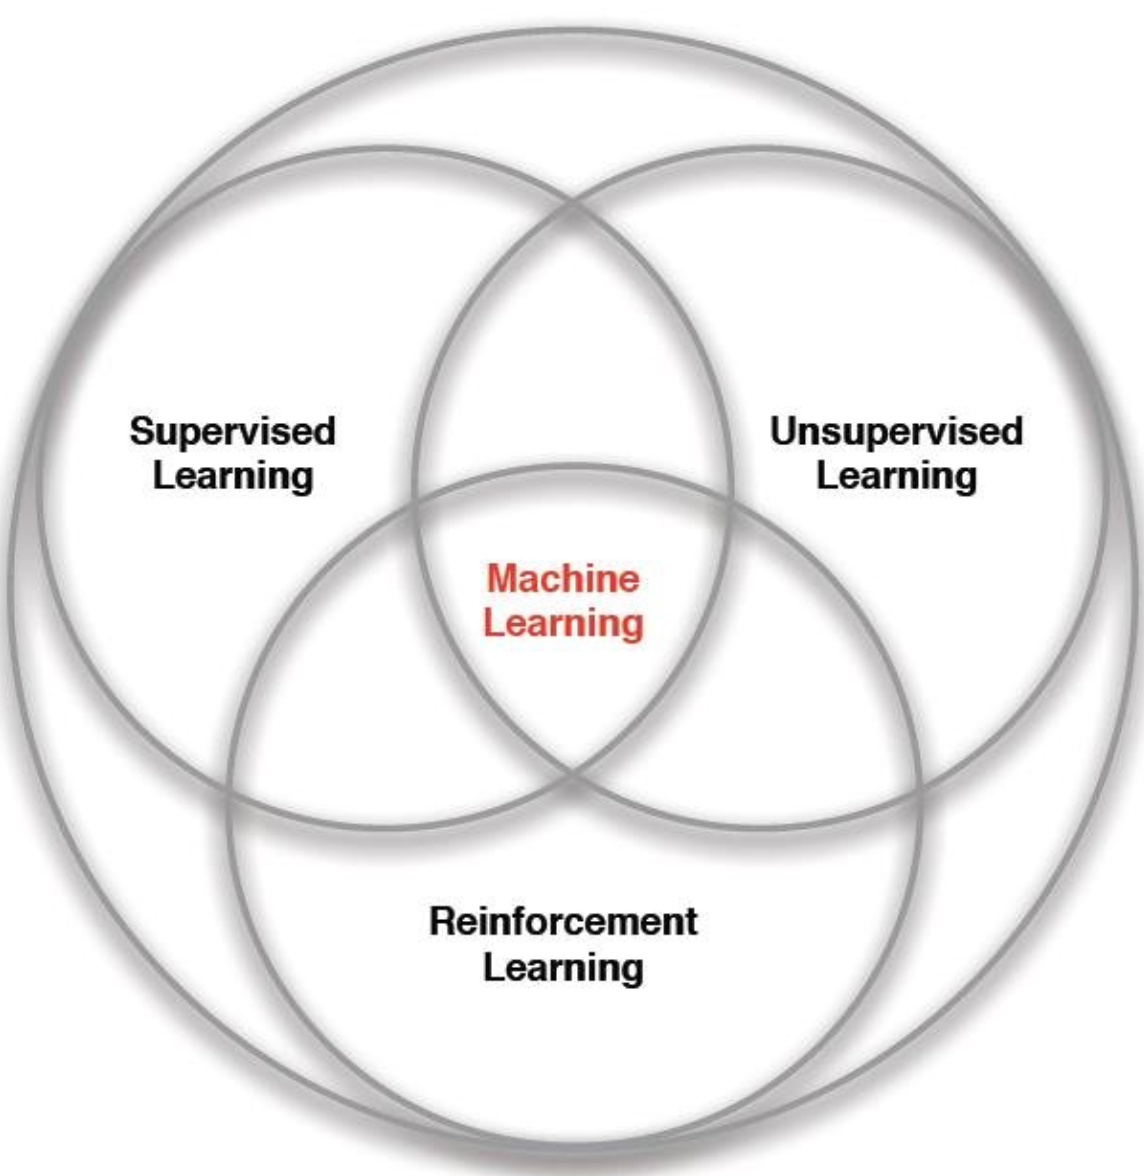
\includegraphics[width=0.5\textwidth]{images/chap2/ML.png}
    \caption{Machine Learning}
    \label{fig:ML}
\end{figure}
\textit{Supervised Learning} is the concept of using previous data to train an algorithm. By training the algorithm on large data-sets, preferable in the order of $10^{4}$ and larger, the goal is to learn the algorithm how to label any new data input. Defining this method in a mathematical sense the algorithm has access to both the input data, $X$, and the output data, $Y$, and tries to model-fit based on these. In example, we would use supervised learning for image classification by allowing the algorithm to train on a large data-set of images (\textit{input}) and labels (\textit{output}). If the algorithm is trained sufficient, the overall goal would be to use a new image as input, and have the algorithm output the correct label.\\\\
\textit{Unsupervised Learning}, on the other hand, is not given data to learn from, but the algorithm is left alone to discover interesting features in the data. Mathematically the algorithm has the input data, $X$, but no information about the output data. This branch of learning can be further divided into two sub-branches; \textit{Association} and \textit{Clustering}. In \textit{Association} the algorithm tries to discover "rules" which describes large portions of the data, in example "when the incident P occurs, L also tends to occur". In \textit{Clustering} the algorithm looks for clusters in the data, in example specific behaviour or trends. 

\section{An introduction to Reinforcement Learning}
In Reinforcement Learning the overall goal is to train an agent, in example an AUV, to perform correct actions in an environment. This is done by giving the agent a \textit{reward} based on how good it was to take a particular \textit{action} in the given state. The reward, $R_{t}$, is defined as a scalar feedback signal, indicating how good it was to take that action at that specific time-step, $t$. The overall goal is to maximise the total cumulative reward over all time-steps in order to find the optimal \textit{policy} to follow, starting in any state. By defining the reward as a scalar signal this means that we assume that every action in the real-world can be weighted against each other, meaning that even ethical dilemmas can be taken into account.\\\\
As stated, the goal of the Reinforcement Learning algorithm is to maximise the total cumulative reward. This is done by taking an action, $A_{t}$, in the environment. An important note her is that taking an action at the time-step $t$ might have a long-term consequence, meaning that the agent don't necessarily experience the consequence of taking that action in the next time-step. This is the same principle as i.e a financial investment.\\\\
In figure \ref{fig:environment} the relationship within Reinforcement Learning is visualised. For each time-step, $t$, the agent will execute an action, $A_{t}$, receive an observation, $O_{t}$ and a scalar reward, $R_{t}$. The environment will receive an action, $A_{t}$, and return an observation, $O_{t}$ and a scalar reward, $R_{t}$ to the agent. 
\begin{figure}[H]
    \centering
    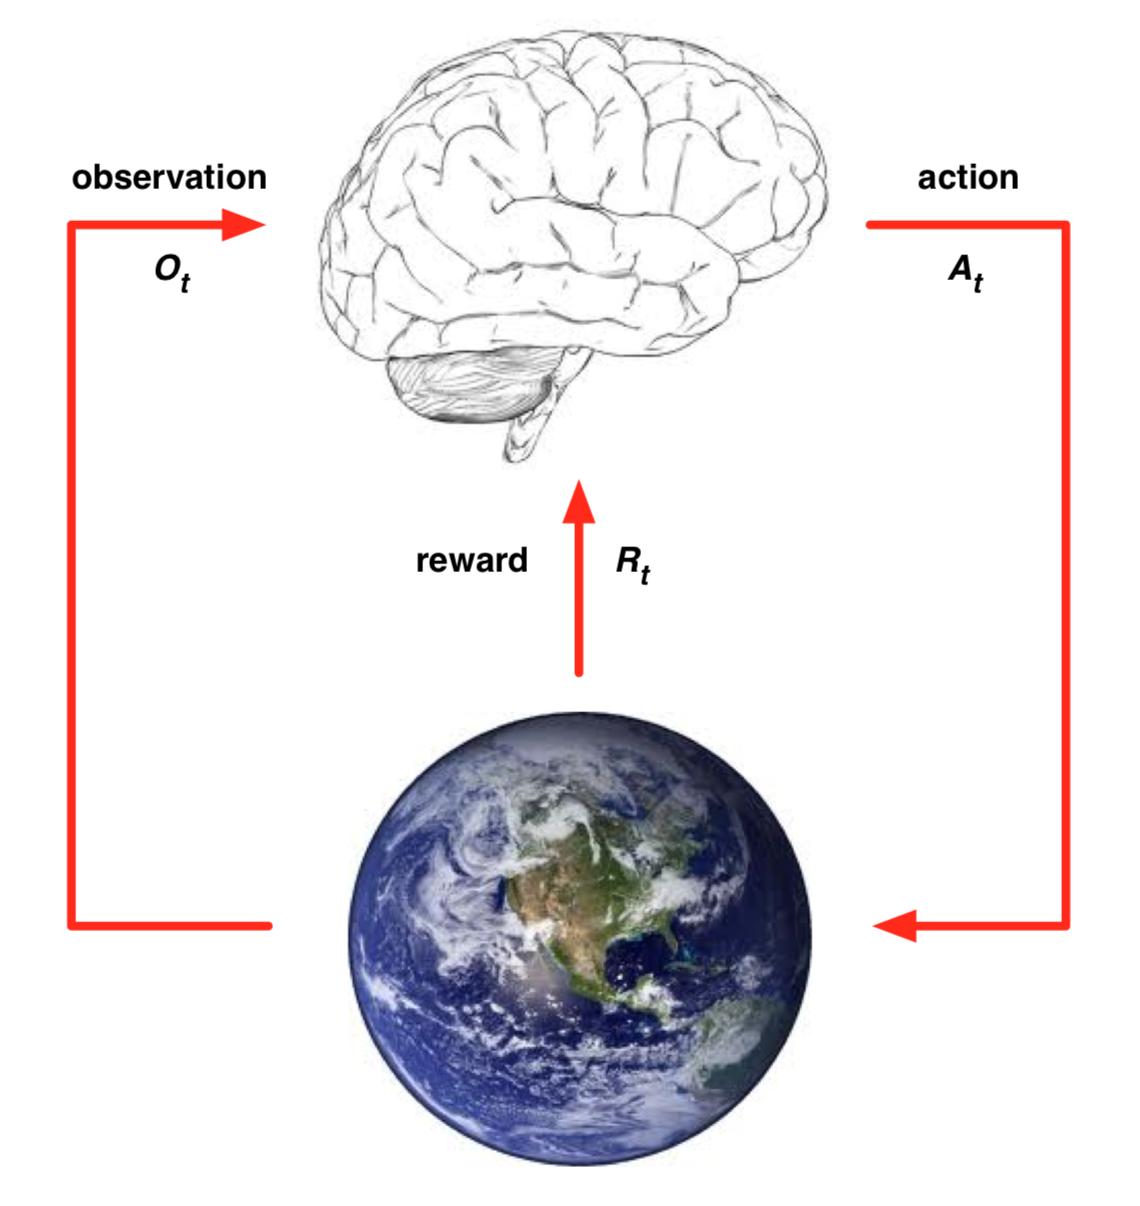
\includegraphics[width=0.5\textwidth]{images/chap2/Agent_environment.png}
    \caption{Reinforced learning environment \cite{Silver}}
    \label{fig:environment}
\end{figure}
\subsection{Markov Decision Processes}
When introducing the concepts of Reinforcement Learning it is necessary to determine what types of \textit{environments} that are possible to "solve" using this technique. A \textit{Markov Decision Process} (MDP) describes a fully $observable$ environment for Reinforcement Learning. A given state, $S_{t}$, is said to be $Markov$ if and only if
\begin{equation}
    P[S_{t+1}] = P[S_{t+1} | S_{1},...,S_{t}]
\end{equation}
In all generality the $\textit{Markov Property}$ states that \textit{the future is independent of the past given the present}, meaning that the state will capture all the relevant information from the history, but the history may be erased once the state is known.\\\\
In an environment where all states are Markov, a \textit{Markov Decision Process} is a Markov reward process with decision. This is given by a tuple $$<\mathcal{S, A, P, R, \gamma}>$$Where
\begin{itemize}
    \item $\mathcal{S}$ - a finite set of states.
    \item $\mathcal{A}$ - a finite set of actions.
    \item $\mathcal{P}$ - a state transition probability matrix.
    \item $\mathcal{R}$ - a reward function, where $\mathcal{R}^{a}_{s} = \mathbb{E}[R_{t+1}|S_{t}=s, A_{t} = a]$.
    \item $\mathcal{\gamma}$ - a discount factor, $\gamma \in [0, 1]$.
\end{itemize}
The reason for using a discount factor, $\mathcal{\gamma}$, has several advantages. From a mathematical prospective it is convenient to discount, as well as making sure that infinite returns are avoided. Furthermore, there is also an uncertainty about the future that is unknown, and the agent do not know if an immediate reward is more valuable than a future reward. In \textit{Markov Decision Processes} three definitions are essential; the \textbf{policy}, $\pi$, the \textbf{state-value} function, $V_{\pi}(s)$, and the \textbf{action-value} function, $q_{\pi}(s,a)$. 
\begin{itemize}
    \item The \textit{policy}, $\pi$, determines how the agent behaves in the environment, meaning which policy it is following. The policy is dependent on the current state, $S_{t}$, and the action taken, $A_{t}$, in that state. This is defined as
    \begin{equation}
        \pi(a|s) = \mathbb{P}[A_{t}=a | S_{t} = s]
    \end{equation}
    \item The \textit{state-value function}, $V_{\pi}(s)$, is the expected return, $G$, by starting in a state, $s_{t}$, and following a specific policy, $\pi$. The state-value function is defined as 
    \begin{equation}
        V_{\pi}(s) = \mathbb{E}_{\pi}[G_{t}|S_{t}=s]
    \end{equation}
    \item The \textit{action-value function}, $q_{\pi}(s,a)$, takes the action into account. Computing the expected return, $G$, by starting in a state, $s_{t}$, taking an action, $a_{t}$, and following a policy, $\pi$. The action-value function is defined as
    \begin{equation}
        q_{\pi}(s,a) = \mathbb{E}_{\pi}[G_{t}|S_{t}=s, A_{t} = a]
    \end{equation}
\end{itemize}
These three definitions are the essential for optimising the MDP. In order to use them the \textit{Bellman Expectation Equation} \cite{Silver} is introduced, which transforms the
definitions above into a new set of \textbf{solvable} definitions. This means that both the state-value function and the action-value function can be decomposed into an immediate reward plus the discounted value of the successor state. This is given as
\begin{itemize}
    \item \textit{Bellman Expectation Equation} for the state-value function, $V_{\pi}(s)$, is given by
    \begin{align}
        V_{\pi}(s) & = \mathbb{E}_{\pi}[R_{t+1}+\gamma V_{\pi}(S_{t+1})|S_{t}=s] \\
        & = \sum_{a\in \mathcal{A}} \pi(a|s)(\mathcal{R}_{s}^{a}+\gamma \sum_{s'\in \mathcal{S}} \mathcal{P}_{ss'}^{a} V_{\pi}(s'))
    \label{eq:bell1}
    \end{align}
    \item \textit{Bellman Expectation Equation} for the action-value function, $q_{\pi}(s,a)$, is given by
    \begin{align}
        q_{\pi}(s,a) & = \mathbb{E}_{\pi}[R_{t+1}+\gamma q_{\pi}(S_{t+1}, A_{t+1}) | S_{t} = s, A_{t} = a] \\
        & = \mathcal{R}_{s}^{a}+\gamma \sum_{s'\in \mathcal{S}} \mathcal{P}_{ss'}^{a} \sum_{a' \in \mathcal{A}} \pi(a'|s')q_{\pi}(s',a')
    \label{eq:bell2}
    \end{align}
\end{itemize}
By doing this the algorithm is able to look one step ahead based on the current state and the action policy it is following. This concept can be explained through a \textit{Look-ahead tree}, which is illustrated in figure \ref{fig:lookahead}. Overall, this look-ahead tree lets the agent evaluate how "\textit{good}" it is to take a particular action given the current state. 
\begin{figure}[H]
    \centering
    \begin{subfigure}[b]{0.45\textwidth}
        \centering
        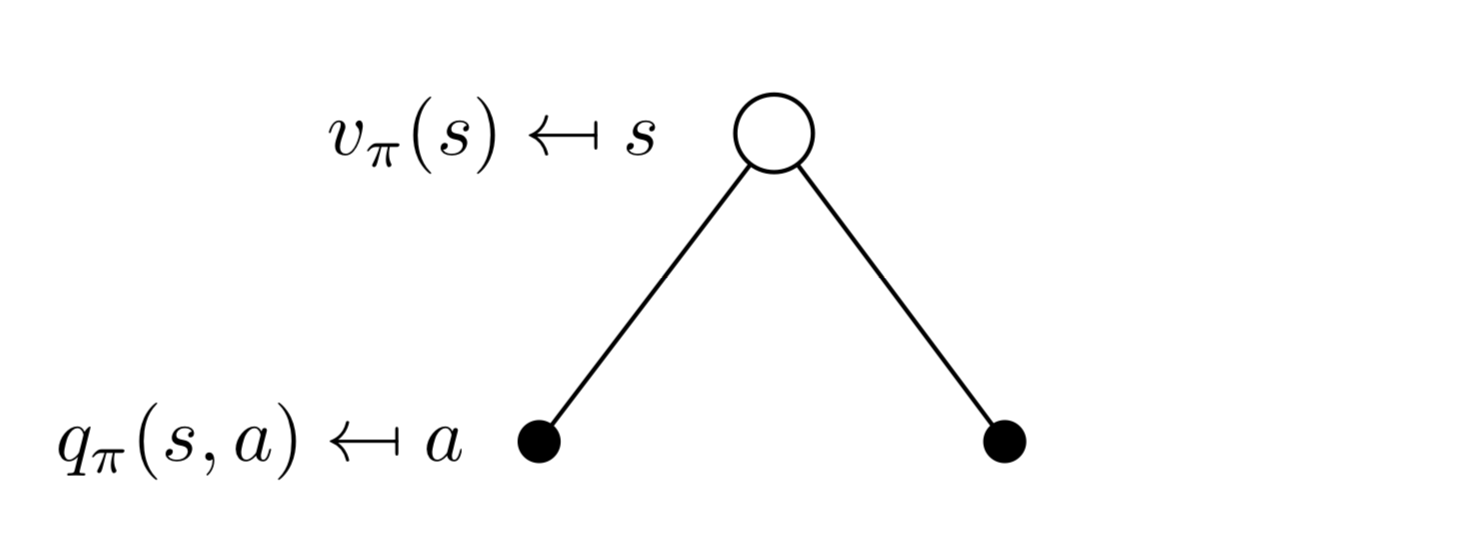
\includegraphics[width=\textwidth]{images/chap2/look-ahead-value.png}
        \caption{state-value function}
    \end{subfigure}
    \hfill
    \begin{subfigure}[b]{0.45\textwidth}
        \centering
        
\includegraphics[width=\textwidth]{images/chap2/look-ahead-action-value.png}
        \caption{action-value function}
    \end{subfigure}
    \caption{Look-ahead tree\cite{Silver}}
    \label{fig:lookahead}
\end{figure}
The overall goal of the MDP is to find the optimal behaviour for the agent, this means that the MDP is "solved" when the agent has found the optimal value function, meaning the best possible policy. This is done by taking the maximum value function, $max_{\pi}$, over both the state-value function and the action-value function. The optimal policy for the agent can then be found by maximising over the optimal action-value function. In conclusion, MDPs, which are environments consisting of a tuple $$<\mathcal{S, A, P, R, \gamma}>$$, is therefore very suitable to solve with Reinforcement Learning. The tuple above also shows that an underwater environment can be defined as an MDP. The state, $S$, would be the location of the AUV in the environment, the action, $A$, would be the direction the AUV is taking in the given state, and the reward, $R$, would say something about how good it is for the AUV to go in this specific direction, based on the objective. By defining the underwater environment as an MDP it shows that Reinforcement Learning can be applied to "solve" problems in the underwater environment.
\subsection{Dynamic Programming}
Solving MDPs often results in a complex and computational costly process, this is where \textit{Dynamic Programming} comes in handy. Dynamic Programming is a method for solving complex problems, where the problem is broken down into sub-problems, and solved separately, before combining the solutions \cite{Silver}. Dynamic Programming works very well for problems with the following properties; \textit{Optimal substructure}, meaning that the problem can be decomposed into $overlapping$ $sub-problems$, resulting in solutions that can be cached and reused. In MDPs, using the Bellman equation results in a recursive decomposition, with the value function both storing and reusing solutions, which means that MDPs satisfies both properties.\\\\
In Reinforcement Learning the dynamic programming algorithm will take the MDP, $<\mathcal{S, A, P, R, \gamma}>$, as input, and return the optimal value function, $V_{*}$, and an optimal policy, $\pi_{*}$. The way it does this is by iterative apply the Bellman Expectation Equations from equation \ref{eq:bell1} and \ref{eq:bell2}. This is done by starting of with an arbitrary initial value function, and sweep over all states in each iteration. The policy is improved by acting $greedily$ with respect to $V_{\pi}$, given by $\pi'=greedy(V_{\pi})$. This concept is illustrated in figure \ref{fig:greedily}. The algorithm initialises an arbitrary state-value and policy function, then it evaluate these, and act greedily to receive an improved state-value and policy function. By iterative doing this the policy will \textbf{always} converge to the optimal value-function, $V^{*}$, and the optimal policy, $\pi^{*}$. 
\begin{figure}[H]
    \centering
    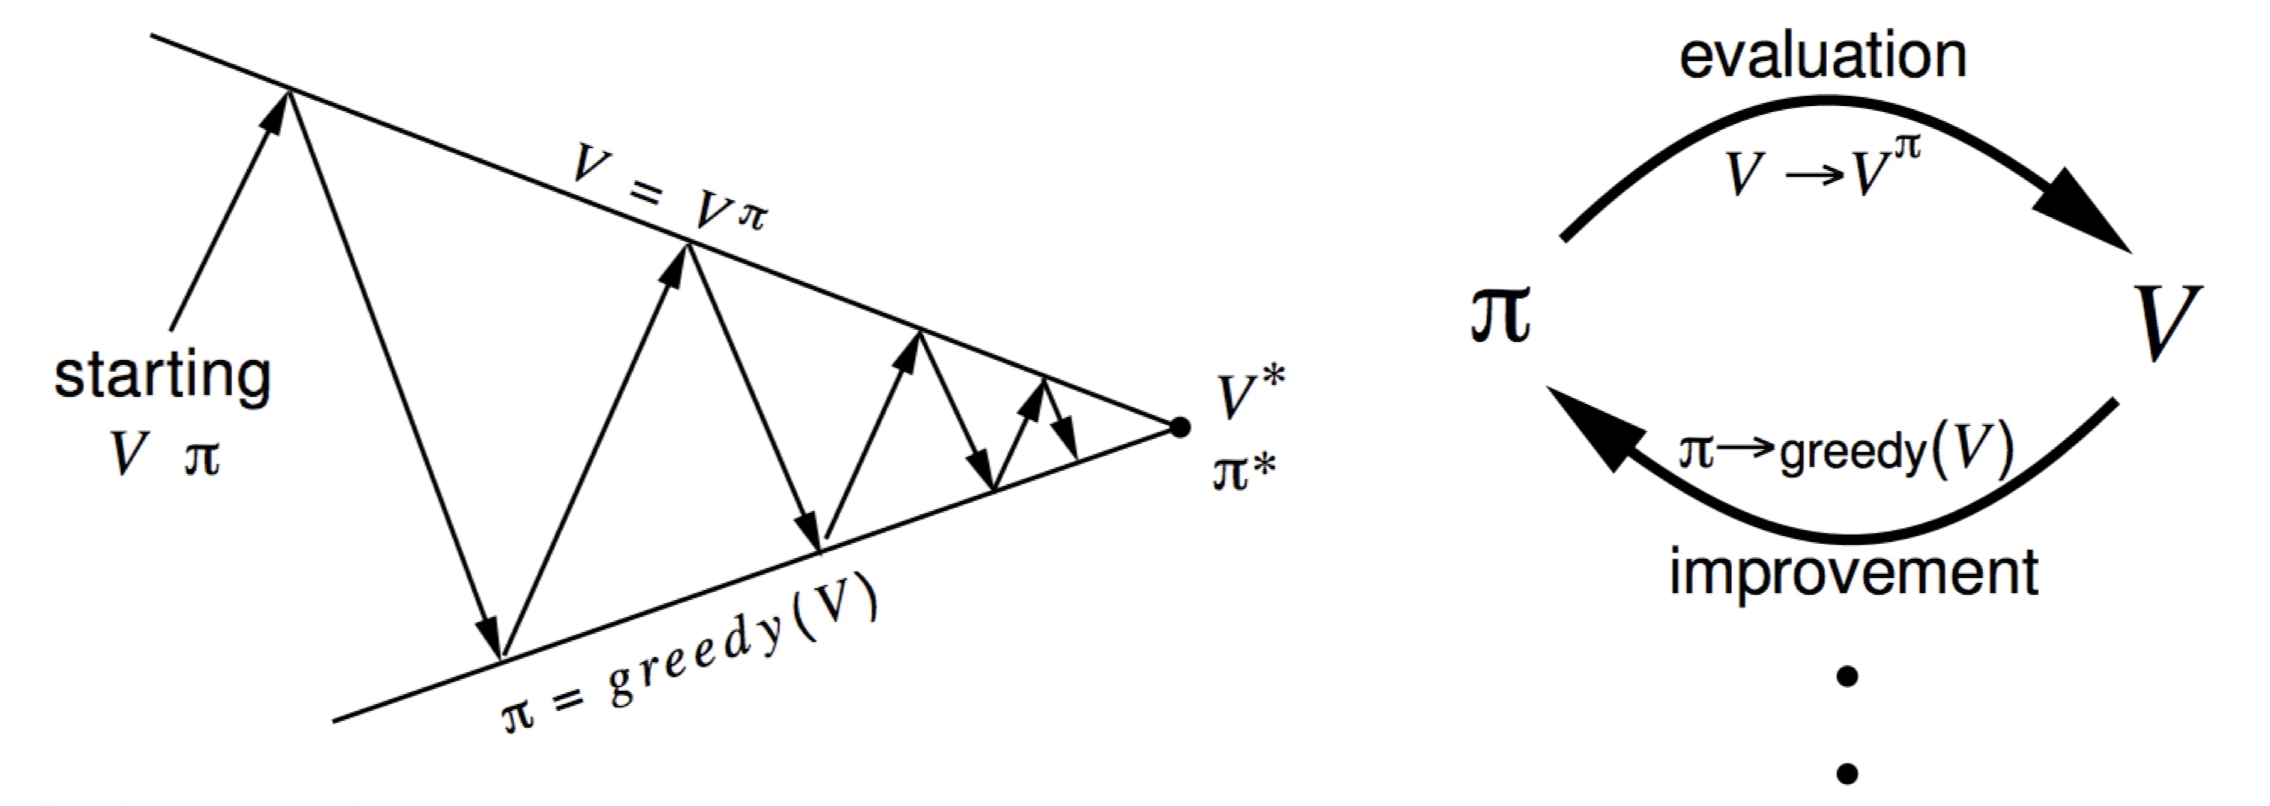
\includegraphics[width=0.75\linewidth]{images/chap2/policy-iteration.png}
    \caption{Policy iteration by acting greedily\cite{Silver}}
    \label{fig:greedily}
\end{figure}

\section{Visual servoing}
The purpose of \textit{Visual servoing} techniques is to control a dynamic system, such as an AUV, by extracting information from a vision sensor \cite{Quentin}. Through the use of multiple cameras the agent is able to extract detailed information about the environment, in the same way as humans. Classical approaches of visual servoing are based on extracting, tracking and matching a set of visual features; points, lines or moments, which are used to move the unit towards a desired pose by using them as input in a control law. \\\\
Extracting, tracking and matching these visual features are a complex task, much because of the high-fidelity information from cameras. In \cite{Collewet} Photometric visual servoing, a method with no feature extraction requirements, was introduced as a possible solution to resolve the complexity of the task. However, compared to classical approaches this solution has a very small convergence domain because of the high non-linearity's between the 3D unit motion and image information. Other, more optimistic, solutions to the problem have centred around using \textit{neural networks}. Deep neural networks, especially \textit{Convolutional Neural Networks} (CNN), have during the recent years contributed to a great leap in a number of computer vision tasks, including: image classification \cite{Hinton}, depth map prediction \cite{Eigen} and real-time 6-DOF camera relocalization \cite{Kendall}. In order to get a better understanding of how the neural networks can be used in robotics it is reasonable to discover how these convolutional networks operates. 
\subsection{Convolutional Neural Networks}
\textbf{Artificial Neural Networks} (ANNs) are based on the idea of how biological nervous systems, such as the human brain, operates \cite{Keiron}. The basic idea of ANNs are to process neurons, interconnected computational nodes, to learn from the input in order to optimise the output. In figure \ref{fig:ann} a common ANN architecture is illustrated, with an \textit{input layer}, a \textit{hidden layer} and an \textit{output layer}. Here the input layer, which usually takes in a multi-dimensional vector, will distribute to the hidden layers, which will make decisions based on the previous layer and see how this improves or detriments the output. This is called the process of learning, and by having multiple hidden layers we commonly refer to it as \textit{deep learning} \cite{McClelland}.
\begin{figure}
    \centering
    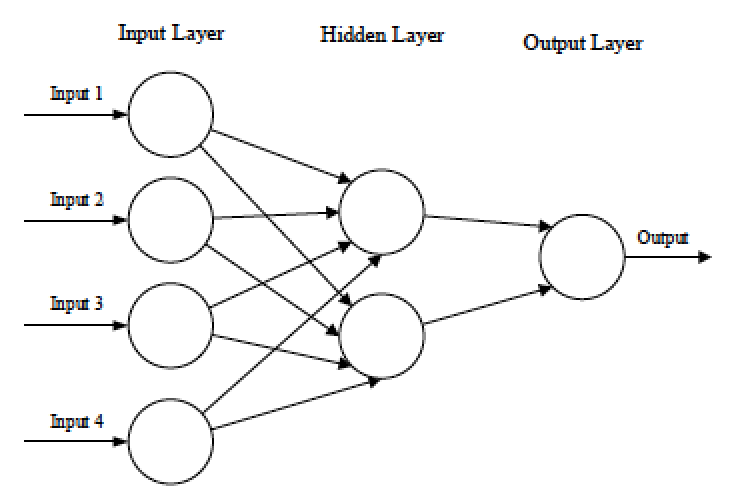
\includegraphics[width=0.7\textwidth]{images/chap2/ANN.png}
    \caption{Common ANN architecture }
    \label{fig:ann}
\end{figure}
\textbf{Convolutional Neural Networks} (CNNs) is based on the same principles of using neurons that self-optimise through learning, as traditional ANNs. As in ANNs each neuron receives an input and perform a operation, and the journey from the raw image vectors to the final score is still being expressed as a single perceptive score function, while the last layer contains loss functions in relation to the classes.\\\\
CNNs differs from ANNs in the way that they are mainly used within pattern recognition in images. The advantage of using these is that they allows us to encode features specific for the image into the architecture, which makes the network better for image-specific tasks.  
\subsubsection{CNN architecture}
In figure \ref{fig:cnn} a simple overview of the relevant components in CNN architecture is visualised. In general the CNN architecture can be divided into three types of layers
\begin{enumerate}
    \item The \textbf{convolutional layer} will apply a convolution operation, which reduces the number of free parameters, to the input, and sends the results to the next layer. The reason for applying the ReLu (\textbf{rectified linear unit}) layer in figure \ref{fig:cnn} is to apply an element-wise activation function to the output from the previous layer. 
    \item The \textbf{pooling layer} continues to reduce the number of parameters, by performing down-sampling along the spatial dimensional of the input from the convolutional layer. 
    \item The \textbf{fully-connected layers} completes the process by attempting to construct class scores from the activations, in order to classify the output. 
\end{enumerate}
\begin{figure}[H]
    \centering
    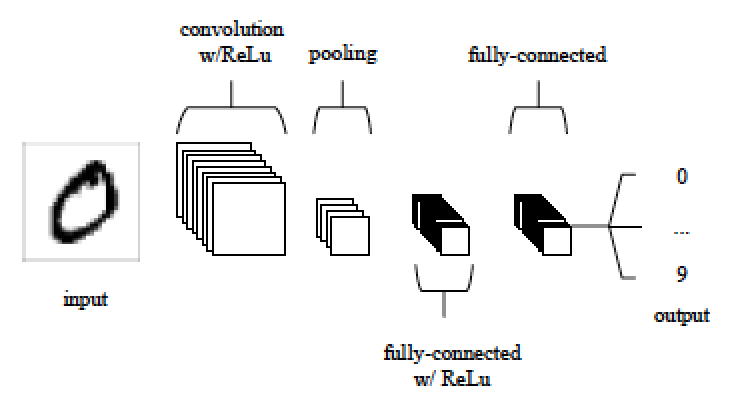
\includegraphics[width=0.7\linewidth]{images/chap2/CNN.png}
    \caption{CNN architecture \cite{Keiron}}
    \label{fig:cnn}
\end{figure}
The overall advantage of having this architecture when applying CNN to image classification problems is that any image can be defined on a \textit{matrix form}, making the layers defined above very intuitive to use. 
\subsubsection{Convolutional layer}
The \textbf{convolutional layer}, which is visualised in figure \ref{fig:convolutional}, aims to detect specific features in the image input, by the use of learnable \textbf{kernels}, which are filters with spatial dimensionality that spreads along the entire image input. Each kernel will produce a 2D activation map when the input makes impact with the layer, and the scalar product is then calculated for each kernel value. The weights of the kernel determines what specific feature that is detected, and our network therefore learns the specific feature based on which kernels that are "firing" activation maps. The kernels that "fires" are defined as \textbf{activations}, and the activation map from each kernel will be placed along the entire depth dimension of the input, to make the full output volume from the layer.
\begin{figure}[H]
    \centering
    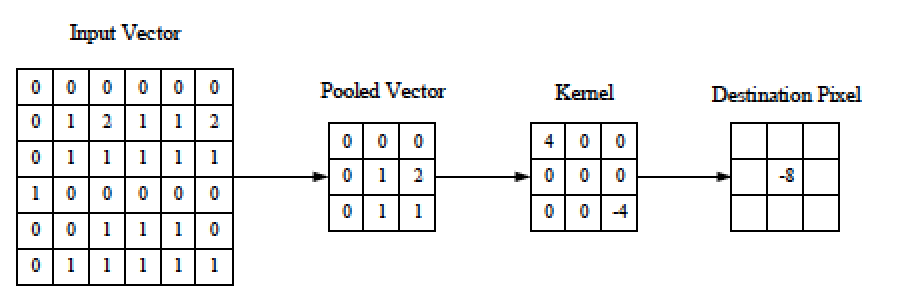
\includegraphics[width=0.7\textwidth]{images/chap2/convolutional_layer.png}
    \caption{Convolutional layer architecture \cite{Keiron}}
    \label{fig:convolutional}
\end{figure}
As shown in figure \ref{fig:convolutional} the centre element of the kernel matrix is placed over the input vector, which then calculates the scalar product and is replaced by a weighted sum based on the neighbour pixels. In the beginning of the section it was stated that ANNs are ineffective on image recognition because of the data size, and thereby the computational power needed to train effectively. The reason for this was that ANN neurons are defined in a fully-connected manner. To resolve this the convolutional layer in CNNs are only connected to a \textit{small} volume of the input, and the dimension of this volume is usually referred to as the \textbf{receptive field size} of the neuron. To see how this resolves the computational complexity we can look at an 64 x 64 x 3 input image, which is an \textit{RBG} image with dimension of 64 x 64. If the receptive field size is set as 6 x 6 this would result in $6*6*3=108$ weights on each neuron, but if we used the same input with standard ANNs it would contain $64*64*3=12,1288$ weights.\\\\
The convolutional layers uses three optimisation hyper-parameters in order to reduce the complexity of the output; \textbf{depth}, \textbf{strides} and \textbf{zero-padding}.
\begin{itemize}
    \item The \textbf{depth} of the output is manually set based on the number of neurons within the layer, by reducing this parameter we can minimise the total number of neurons in the network and reduce complexity of the output. However, there is a trade-off in doing this, since less neurons also results in reduced pattern recognition capabilities.
    \item The \textbf{stride} of the output, which is the depth surrounding the spatial dimensionality that places the receptive field, can also be set manually. In example, by choosing this equal to 1 it would produce large activations, because we have heavily overlapping receptive fields. Increasing the stride will however reduce the overlapping and result in lower spatial dimensions.
    \item The \textbf{zero-padding} means "padding" the input border, which gives us further control of the output volume dimension.
\end{itemize}
All these optimisation parameters will impact the spatial dimensionality of the output from the convolutional network. The impact can be calculated by
\begin{equation}
    \frac{(V-R)+2Z}{S+1}
\label{eq:spatial}
\end{equation}
where V is the input volume, R is the receptive field size, Z the amount of zero-padding and S is the stride \cite{Keiron}. The output of equation \ref{eq:spatial} needs to be equal to an integer. If this is not the case the stride has been defined wrong, meaning that the neurons will not be able to fit smoothly across the input. 
\subsubsection{Pooling layer}
The output from the convolutional layer will be sent further on to the \textbf{pooling layer}. The pooling layer will further reduce the dimension of the input through reducing the computational complexity and the number of parameters.\\\\
This is done through the use of a \textbf{max} function, which usually is defined with kernels of dimension 2 x 2 and a stride of 2 along the spatial dimension of the input. Overall, the use of a pooling layer will reduce the activation map with $\approx$ 75 percent of the original size, while still maintaining the depth of the input volume. This reduction can be seen in figure \ref{fig:convolutional}. 
\subsubsection{Fully-connected layers}
Finally the \textbf{fully-connected layer} is attached at the end of the network. In all simplicity this layer will take in an input volume from the convolutional layer, ReLu or the pooling layer, and output a vector specifying the number of detection classes the program can choose from, i.e cat, dog, etc. 



\chapter{Station Keeping of AUVs with Reinforced learning} \label{chap:station-keeping}
Traditional Station Keeping of AUVs and ROVs are usually based around \textbf{PID}, proportional-integral-derivative, algorithms. In all simplicity the PID controller is a control-loop feedback algorithm, which continuously calculates an error value between a specified desired position and the actual position of the vehicle. The PID algorithm is given in equation \ref{eq:pid}, where $K_{p}$, $K_{i}$ and $K_{d}$ denote the coefficients for the proportional, integral and derivative gains, respectively. 
\begin{equation}
\centering
{\displaystyle \tau = K_{\text{p}}e(t)+K_{\text{i}}\int _{0}^{t}e(\tau )d\tau +K_{\text{d}}{\frac {d(t)}{dt}}}
\label{eq:pid}
\end{equation}
The algorithm uses the \textbf{proportional} term to reduce the error, the \textbf{integral} term to remove possible stationary deviation and the \textbf{derivative} term takes the error values rate of change into account, and thereby tries to compensate for future trends of error.\\\\
To accomplish a sufficient PID algorithm for a given system the controller gains needs to be tuned. The methods of tuning a PID algorithm are many \cite{Fossen}, but they usually surrounds using the mass- and damping-matrices of the system, as well as defining the natural frequency, $\omega_{n}$, and the natural damping, $\zeta$, resulting in \textbf{constant} gains. However, the underwater environment is complex, and the autonomous control of AUVs is nonlinear, because of their motions being highly affected by both flow and hydraulic resistance. This results in accurate control being very difficult, especially when the PID algorithm uses constant gains.\\\\
During the recent years there has been a rapid development of artificial intelligence, and machine learning is now being widely used within control theory. The overall goal of using AI in control is to solve complex tasks from unprocessed, high-dimensional and sensory input \cite{Lillicrap}, and several propositions has been made for doing this. David Silver et al. proposed using a \textbf{DPG}, Deterministic Policy Gradient algorithm, for performing complex tasks with high dimensionality, which showed significantly better performance than using stochastic policy gradients as well as having usage on nonlinear optimisation problems \cite{David}. Furthermore Yu Runsheng et al. proposed in 2017 the use of a \textbf{DDPG}, Deep Deterministic Policy Gradient, for trajectory tracking control of AUVs \cite{Yu}, which showed significant improvement compared to the traditional PID controllers. The experiments done in \cite{Yu} and \cite{David} are therefore used as a starting point for accomplishing Station Keeping of AUVs based on Reinforcement Learning.
\section{Deep Deterministic Policy Gradient algorithm}
The Deep Deterministic Policy Gradient (DDPG) algorithm is an \textbf{off-policy}, \textbf{model-free}, \textbf{policy-gradient} and \textbf{actor-critic} algorithm \cite{Emami}. The fact that it is a \textit{policy-gradient} means that it tries to optimise a \textit{policy}, which was defined in chapter \ref{chap: deep}, end-to-end by computing noisy estimates from the gradient of the expected reward from following that specific policy, and then updating the policy in the gradient direction. By being \textit{actor-critic} we recall from chapter \ref{chap: deep} that the policy function (\textit{actor}) is independent of the value function (\textit{critic}). The policy function takes an action in the current state, and the value function computes a \textit{Temporal Difference} (TD) error signal based on the current state and the reward from taking that action. Furthermore, the algorithm is \textit{off-policy} meaning that the policy function is updated every time-step, without making any assumptions if whether or not the agent are following the actual policy.\\\\Finally, by being \textit{model-free} the algorithm do not know anything about the underlying dynamics of how the AUV interacts with the environment. The benefit of doing this is that the model-free algorithms will directly estimate an optimal policy or a value function through the use of a policy iteration or value iteration. This reduces the computational power needed and complexity of the problem significantly compared to \textit{model-based} approaches. Obviously it is more complex to have a model-free approach, in the sense that we require a larger number of training examples, so starting of with a good approximation of the underlying model of the environment is beneficial. However, if the approximation is far off it will only make the problem worse.
\subsection{Exploration and Exploitation}
An important note when dealing with DDPG algorithms, and Reinforcement Learning in general, is the relationship between \textbf{exploration} and \textbf{exploitation}. This involves the trade-off between exploitation, meaning that the agent uses the "learned" best action to take in a given state, and exploration, meaning that the agent "tries" a new action in a given state. This deals with the fact that although the agent has found what it believes to be the optimal action in a given state, there could always exist an unexplored action that is better. The possibility for exploration is therefore implemented, in order to avoid a \textit{sub-optimal} policy.\\\\
The trade-off between exploration and exploitation is usually determined by a parameter, $\epsilon$. If $\epsilon \longrightarrow 0$ the agent will only exploit previous learned optimal policies, and if $\epsilon \longrightarrow 1$ the agent will always explore new actions in a given state. When the agent is starting to explore the environment, it will have no prior knowledge about it. This means that it should both explore and exploit actions. However, as the agent discovers more about the environment, meaning that it increases its \textit{situational awareness}, the probability of the "learned" action being the optimal will increase. This means that $\epsilon$ should decrease as the knowledge about the environment increases. 






\include{chapter32}
\chapter{Modeling} \label{chap:modeling}
The simulations will be conducted using the \textbf{BlueROV2} by \textit{BlueRobitcs} \cite{blue}. The BlueROV2 has a 6-thruster vectored configuration, open-source electronics and software, and works well for inspections, research, and adventuring. The simulation model does not include the BlueROVs' tether, which connects the vehicle to i.e a surface vessel, which means that the vehicle is modelled as an AUV. 
\begin{figure}[H]
    \centering
    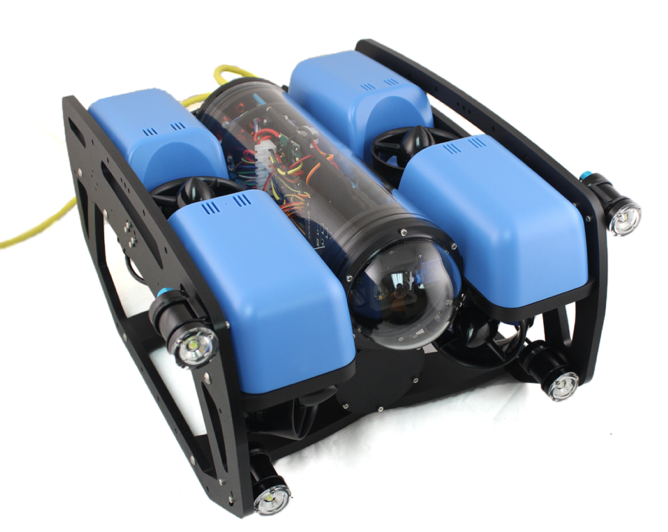
\includegraphics[width=0.7\textwidth]{images/chap4/bluerov2.png}
    \caption{BlueROV2 by BlueRobotics \cite{blue}}
    \label{fig:bluerov2}
\end{figure}
\section{Reference frames}
\begin{figure}[H]
    \centering
    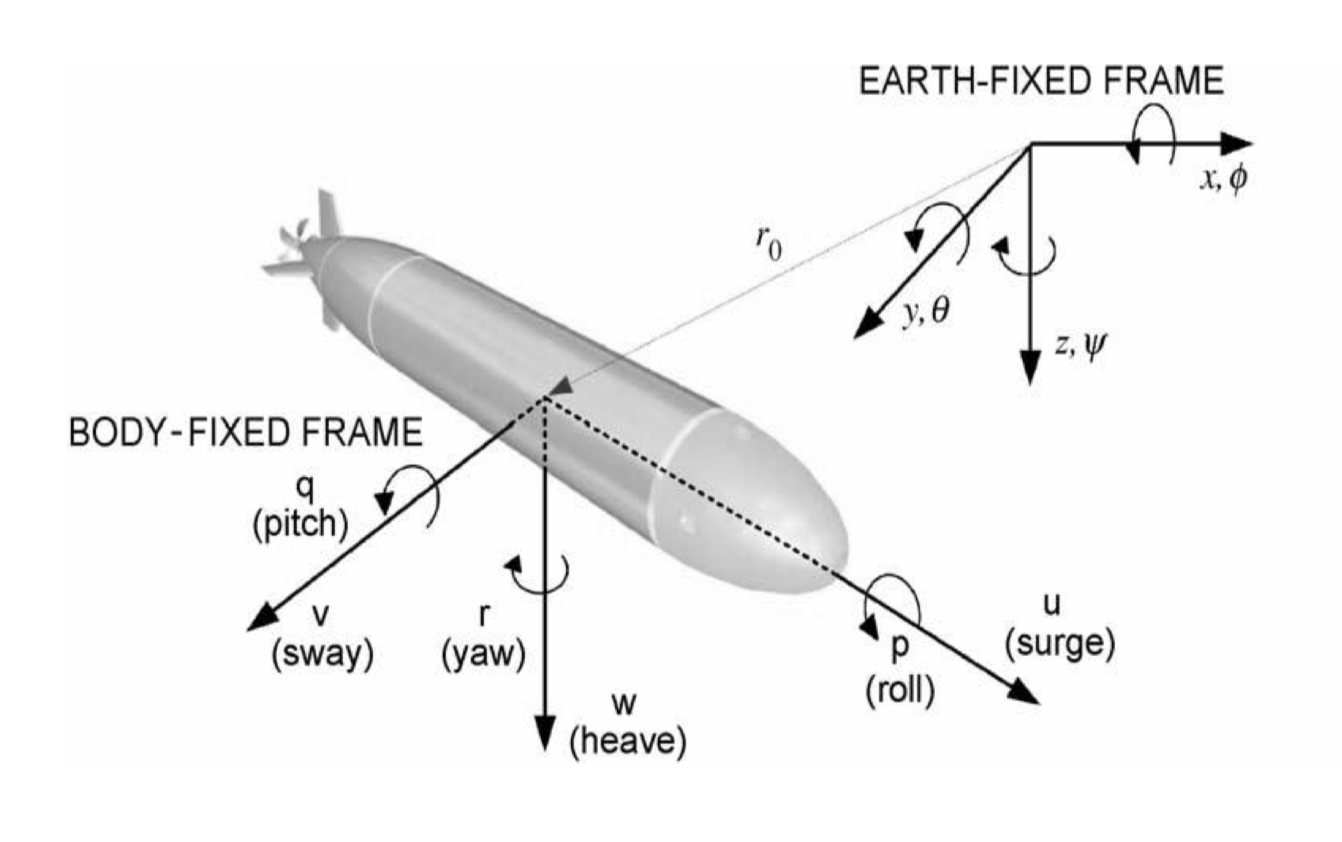
\includegraphics[width=0.7\textwidth]{images/chap4/reference_frames.png}
    \caption{Body fixed and earth fixed reference frame}
    \label{fig:reference_frame}
\end{figure}
In figure \ref{fig:reference_frame} the BlueROV2s' 6 degrees of freedom (DOFs) in the \textbf{Body-fixed} and \textbf{Earth-fixed} reference frame are illustrated. Here the \textbf{North-East-Down} (NED) reference frame will be used as the earth-fixed reference frame. When analysing motion in 6 DOFs it is convenient to define motion in different reference, or coordinate, frames. The reference frames are given by
\begin{itemize}
    \item \textit{NED} is defined as a coordinate system $\{n\} = (x_{n},y_{n},z_{n})$ with origin $o_{n}$ relative to the Earth's reference ellipsoid, commonly defined as the tangent plane to the surface of the Earth moving with the vessel \cite{Fossen}. Here, the $x_{n}$ axis points towards true North, the $y_{n}$ axis points towards the true East and the $z_{n}$ axis points downwards normal to the surface. 
    \item \textit{Body} is defined as a coordinate system $\{b\} = (x_{b},y_{b},z_{b})$ with origin $o_{b}$ centred at the vessels centre of mass, and moving with the body. Here, the $x_{b}$ axis is directed from aft to fore, the $y_{b}$ transverse axis is directed towards starboard and the $z_{b}$ normal axis directed from top to bottom. 
\end{itemize}
The notations in figure \ref{fig:reference_frame} are defined according to SNAME (1950) \cite{Fossen}, which is given in figure \ref{fig:sname}. The SNAME notation will be used throughout this paper. 
\begin{figure}
    \centering
    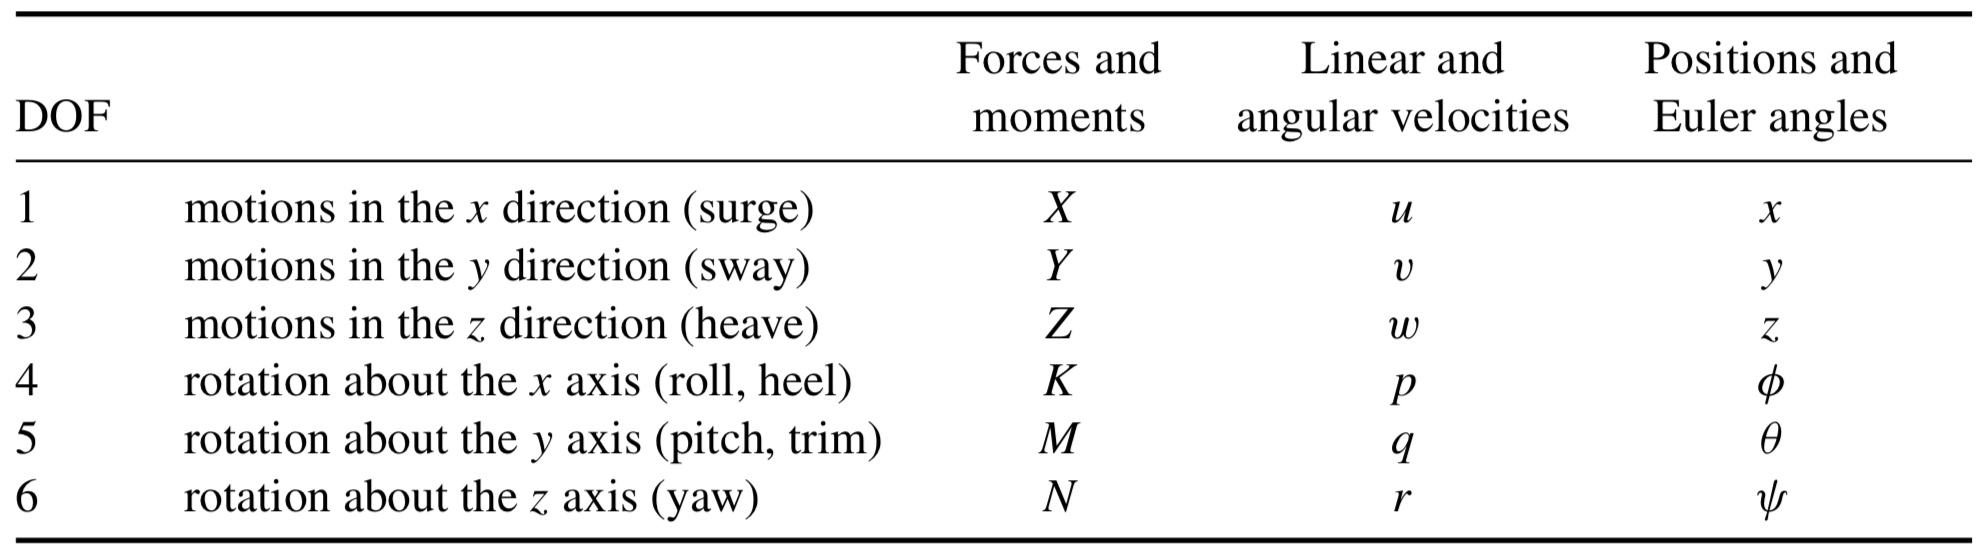
\includegraphics[width=\textwidth]{images/chap4/SNAME.png}
    \caption{The notation of SNAME (1950) for marine vessels}
    \label{fig:sname}
\end{figure}
\section{Dynamic Model of Underwater Vehicles}
From \textit{Fossen} \cite{Fossen} the underwater dynamic equation of motions can be expressed as
\begin{align}
    M\Dot{v}+C(v)v+D(v)v+g(\mu)+\delta & = \tau \\
    \longrightarrow (M_{RB}+M_{A})\Dot{v}+(C_{RB}(v)+C_{A}(v))v+(D_{L}+D_{Q})v + g(\mu)+\delta & = \tau 
    \label{eq:motion}
\end{align}
For simplicity the external forces, in example environmental forces $\tau_{env}$, are here neglected. $\tau$ is therefore the forced applied by the controller, while $\delta$ is a model uncertainty vector. The terms in equation \ref{eq:motion} are defined in the following sections.
\subsection{Mass matrix}
The Mass matrix consist of the rigid-body terms and the hydrodynamic mass terms. The hydrodynamic terms are due to \textit{added mass}, which is mass created by the acceleration of the surrounding water when a vehicle is moving through a stationary fluid \cite{Fossen}. 
\begin{align}
    \textbf{M}_{RB} & = \begin{bmatrix}
                m*I_{3x3} & 0_{3x3}\\
                0_{3x3} & I_{g}
                \end{bmatrix} \\
    \mathbf{I}_{g} & = \begin{bmatrix}
                I_{x} & -I_{xy} & -I_{xz} \\
                I_{yx} & I_{y} & -I_{yz} \\
                -I_{zx} & -I_{zy} & I_{z}
                \end{bmatrix} \\
    \textbf{M}_{A} & = \begin{bmatrix}
                X_{\Dot{u}} & X_{\Dot{v}} & X_{\Dot{\omega}} & X_{\Dot{p}} & X_{\Dot{q}} & X_{\Dot{r}} \\
                Y_{\Dot{u}} & Y_{\Dot{v}} & Y_{\Dot{\omega}} & Y_{\Dot{p}} & Y_{\Dot{q}} & Y_{\Dot{r}} \\
                Z_{\Dot{u}} & Z_{\Dot{v}} & Z_{\Dot{\omega}} & Z_{\Dot{p}} & Z_{\Dot{q}} & Z_{\Dot{r}} \\
                K_{\Dot{u}} & K_{\Dot{v}} & K_{\Dot{\omega}} & K_{\Dot{p}} & K_{\Dot{q}} & K_{\Dot{r}} \\
                M_{\Dot{u}} & M_{\Dot{v}} & M_{\Dot{\omega}} & M_{\Dot{p}} & M_{\Dot{q}} & M_{\Dot{r}} \\
                N_{\Dot{u}} & N_{\Dot{v}} & N_{\Dot{\omega}} & N_{\Dot{p}} & N_{\Dot{q}} & N_{\Dot{r}} \\
                \end{bmatrix} \\
\end{align}
where \textbf{m} denotes the total mass of the ROV, and \textbf{I$_{x}$, I$_{y}$, I$_{z}$} represents the moment of inertia about the body axis. Because of symmetry the products of inertia, here represented on the off-diagonal, will have the form \textbf{I$_{xy}$} = \textbf{I$_{yx}$}, \textbf{I$_{yz}$} = \textbf{I$_{zy}$} and \textbf{I$_{zx}$} = \textbf{I$_{xz}$}. The added mass matrix consist of hydrodynamic derivatives, which is given by
\begin{equation}
N_{\Dot{k}} = \frac{\partial N}{\partial \Dot{k}}
\end{equation}
where N = ($X, Y, Z, K, M, N$) and k = ($u, v, \omega, p, q, r$). In example, $X_{\Dot{u}}$ represent the added mass force coefficient in surge due to an acceleration in surge.
\subsection{Coriolis and Centripetal force matrices}
The Coriolis-Centripetal matrix will also consist of a rigid-body and hydrostatic term. From Fossen \cite{Fossen} the rigid-body Coriolis-Centripetal matrix can be found by defining $\textbf{M}_{RB}$ as
\begin{equation}
    \mathbf{M}_{RB} = \mathbf{M}_{RB}^{T} = \begin{bmatrix}
    \mathbf{M}_{11} & \mathbf{M}_{12} \\
    \mathbf{M}_{21} & \mathbf{M}_{22}
    \end{bmatrix} > 0
\end{equation}
where $\textbf{M}_{21}=\textbf{M}_{12}^T$. $\mathbf{C}_{RB}$ is then found by
\begin{equation}
    \mathbf{C}_{RB}(\mathbf{\nu}) = \begin{bmatrix}
    0_{3x3} & -S(M_{11}\nu_{1}+M_{12}\nu_{2}) \\
    -S(M_{11}\nu_{1}+M_{12}\nu_{2}) & -S(M_{21}\nu_{1}+M_{22}\nu_{2})
    \end{bmatrix}
\end{equation}
where $\nu_{1} := v_{b/n}^{b} = [u, v, \omega]^{T}, \nu_{2} := \omega_{b/n}^{b}=[p, q, r]^{T}$ and $S$ is the cross-product operator. The hydrodynamic Coriolis-Centripetal matrix can be found in the same way, by using $\textbf{M}_{A}$. This yields
\begin{align}
    \mathbf{M}_{A} & = \mathbf{M}_{A}^{T} = \begin{bmatrix}
    \mathbf{A}_{11} & \mathbf{A}_{12} \\
    \mathbf{A}_{21} & \mathbf{A}_{22}
    \end{bmatrix} > 0 \\
    \mathbf{C}_{A}(\mathbf{\nu}) & = \begin{bmatrix}
    0_{3x3} & -S(A_{11}\nu_{1}+A_{12}\nu_{2}) \\
    -S(A_{11}\nu_{1}+A_{12}\nu_{2}) & -S(A_{21}\nu_{1}+A_{22}\nu_{2})
    \end{bmatrix}
\end{align}
\subsection{Damping matrices}
As stated previously the environmental forces are neglected in equation \ref{eq:motion}, which means that skin friction and vortex shedding will dominate the damping term. This leads to the simplified hydrodynamic damping terms in equation \ref{eq:damp} and \ref{eq:damp1}.
\begin{align}
    \mathbf{D}_{L} & = -\begin{bmatrix}
                X_{u} & 0 & 0 & 0 & 0 & 0\\
                0 & Y_{v} & 0 & 0 & 0 & 0 \\
                0 & 0 & Z_{\omega} & 0 & 0 & 0 \\
                0 & 0 & 0 & 0 & K_{p} & 0 & 0 \\
                0 & 0 & 0 & 0 & 0 & M_{q} & 0 \\
                0 & 0 & 0 & 0 & 0 & 0 & N_{r} 
                \label{eq:damp}
                \end{bmatrix} \\
    \mathbf{D}_{Q} & = -\begin{bmatrix}
                X_{u|u|}|u| & 0 & 0 & 0 & 0 & 0\\
                0 & Y_{v|v|}|v| & 0 & 0 & 0 & 0\\
                0 & 0 & Z_{\omega|\omega|}|\omega| & 0 & 0 & 0\\
                0 & 0 & 0 & K_{p|p|}|p| & 0 & 0 \\
                0 & 0 & 0 & 0 & M_{q|q|}|q| & 0 \\
                0 & 0 & 0 & 0 & 0 & N_{r|r|}|r|
                \label{eq:damp1}
                \end{bmatrix}|\mathbf{v}| \\
\end{align}
\subsection{Hydrostatic terms}
The hydrostatic matrix, $g(\mu)$, accounts for the restoring forces, which is defined as the relationship between weight, W, and buoyancy, B. By assuming that the vehicle is neutrally buoyant it will satisfy $W = B$, and by further assuming that the \textit{centre of gravity} (COG) and the \textit{centre of buoyancy} (COB) are located vertically on the $z$ axis, the hydrostatic matrix can be defined as in \cite{Fossen}
\begin{equation}
    g(\mu) = [0, 0, 0, \Bar{BG}_{z} W cos(\phi)sin(\phi), \Bar{BG}_{z} W sin(\theta), 0]^{T}
\end{equation}
where $\Bar{BG}_{z}=z_{g}-z_{b}$, with $z_{g}$ being the $z$ component in COG, and $z_{b}$ being the $z$ component in COB, and $\mu = [N, E, D, \phi, \theta, \psi]$ in the (NED) and (Body) reference frames. 
\chapter{Method} \label{chap:method}
\section{Controller implementation for the BlueROV2}
The \textbf{BlueROV2} has 13 states, which are defined hereafter as
\begin{itemize}
    \item 3 \textit{position} states defined in the (NED) frame as [$x$, $y$, $z$]
    \item 4 \textit{orientation} states defined in the (NED) frame as the quaternions [$\epsilon_{1}$, $\epsilon_{2}$, $\epsilon_{3}$, $\eta$]
    \item 3 \textit{linear velocity} states defined in the (Body) frame as [$u$, $v$, $w$]
    \item 3 \textit{angular velocity} states defined in the (Body) frame as [$p$, $q$, $r$]
\end{itemize}
The orientation states are defined as \textit{quaternions} in order to resolve the issue connected to singularity in $\theta = \pm 90 \deg$ when using \textit{Euler angles}. However, when we are to use these states in the controller we need to transform them into Euler angles. The singularity wont be an issue when doing this, since the transformation don't affect the model. From (eq. 2.58) in Fossen \cite{Fossen} we have that the rotation matrix from (BODY) to (NED) for the quaternions is defined as
\begin{equation}
    \mathbf{R}_{b}^{n}(\mathbf{q}) = 
    \begin{bmatrix}
    1 - 2(\epsilon_{2}^{2}+\epsilon_{3}^{2}) & 2(\epsilon_{1}\epsilon_{2}-\epsilon_{3}\eta) & 2(\epsilon_{1}\epsilon_{3}+\epsilon_{2}\eta) \\
    2(\epsilon_{1}\epsilon_{2}+\epsilon_{3}\eta) & 1 - 2(\epsilon_{1}^{2}+\epsilon_{3}^{2}) & 2(\epsilon_{2}\epsilon_{3}-\epsilon_{1}\eta) \\
    2(\epsilon_{1}\epsilon_{3}-\epsilon_{2}\eta) & 2(\epsilon_{2}\epsilon_{3}+\epsilon_{1}\eta) & 1 - 2(\epsilon_{1}^{2}+\epsilon_{2}^{2})
    \end{bmatrix}
\end{equation}
Furthermore we have from (eq. 2.76) in that 
\begin{equation}
    \mathbf{R}_{b}^{n}(\Theta_{nb}) := \mathbf{R}_{b}^{n}(\mathbf{q})
\end{equation}
which gives us that the relationship between the Euler angles, $\phi$, $\theta$ and $\psi$, and the quaternions can be defined as
\begin{equation}
    \begin{bmatrix}
    c\psi c\theta & -s\psi c \phi + c\phi s\theta s\phi & s\psi s\phi + c\psi c\phi s\theta \\ s\psi c\theta & c\phi c\phi + s\phi s\theta s\psi & -c\psi s\phi + s\theta s\psi c\phi \\ -s\theta & c\theta s\phi & c\theta c\phi 
    \end{bmatrix}
    = \begin{bmatrix}
    R_{11} & R_{12} & R_{13} \\ R_{21} & R_{22} & R_{23} \\ R_{31} & R_{32} & R_{33}
    \end{bmatrix}
\end{equation}
here $c = cos$ and $s = sin$. This results in the following Euler angles, which is used in the controller
\begin{align}
    \phi & = atan2(R_{32}, R_{33}) = atan2(2(\epsilon_{2}\epsilon_{3}+\epsilon_{1}\eta), 1 - 2(\epsilon_{1}^{2}+\epsilon_{2}^{2})) \\
    \theta & = -sin^{-1}(R_{31}) = -sin^{-1}(2(\epsilon_{1}\epsilon_{3}-\epsilon_{2}\eta)) \\
    \psi & = atan2(R_{21}, R_{11}) = atan2(2(\epsilon_{1}\epsilon_{2}+\epsilon_{3}\eta), 1 - 2(\epsilon_{2}^{2}+\epsilon_{3}^{2}))
\end{align}
$\phi$ and $\theta$ defines the rotation in surge and sway, respectively. In order to simplify the implementation of a controller based on Reinforcement Learning it is convenient to not include these two in the algorithm. The reason for this is that we are trying to accomplish Station Keeping, and the rotation in surge and sway is not as "important" as the rotation about the z-axis, $\psi$. To further simplify the problem we also neglect the position in $z$, as stated previously, since we are assuming a constant depth.\\\\
Although these three states, $\phi$, $\theta$ and $z$, are not accounted for by the Reinforcement Learning algorithm, meaning that the algorithm do not produce thrust in these directions/orientations, their states will \textbf{affect} the algorithm. In order to resolve this I suggest to first implement a classical control algorithm, in order to make these three states stable on their own, before implementing the Reinforcement Learning algorithm on the resulting states. 
\subsection{Implementation of PD algorithm}
As mentioned in chapter \ref{chap:station-keeping} the PID algorithm is a common method for control, but in most cases only using a PD algorithm will be sufficient. In order to accomplish Station Keeping of the AUV the PD algorithm should adjust thrust in the $z$ direction as well as the $\phi$ and $\theta$ angles. The PD algorithm is thereby given by
\begin{align}
    \tau & = K_{p}e(t) + K_{d}\frac{d(t)}{dt} \\
    \longrightarrow
    \begin{bmatrix}
    \tau_{z}(t) \\ \tau_{\phi}(t) \\ \tau_{\theta}(t) 
    \end{bmatrix}
    & = K_{p} \begin{bmatrix}
    e(t)_{z} \\ e(t)_{\phi} \\ e(t)_{\theta} 
    \end{bmatrix}
    + K_{d} \begin{bmatrix}
    \omega(t) \\ p(t) \\ q(t)
    \end{bmatrix}
\end{align}
\subsection{Implementation of DDPG algorithm}
As mentioned in chapter \ref{chap:station-keeping} the DDPG is a policy-gradient algorithm, which uses a stochastic behaviour policy for good exploration, but estimates a deterministic target policy, which is easy to learn. In order to implement this there will be used two \textbf{neural networks}, a \textit{control} neural network (actor) and an \textit{evaluation} neural network (critic), based on the experiments done by (Yu, Runsheng., et al.) \cite{Yu}.\\\\
In order to define the neural networks we recall the equations of motion of underwater vehicles, defined in equation \ref{eq:motion}. By assuming the rotation in roll direction, $\phi$, and the rotation in pitch direction, $\theta$, small, the rotation matrix from (Body) to (NED) can be defined as
\begin{equation}
    \Re(\psi) = 
    \begin{pmatrix}
    cos(\psi) & -sin(\psi) & 0 \\
    sin(\psi) & cos(\psi) & 0 \\
    0 & 0 & 1
    \end{pmatrix}
\end{equation}
Furthermore, by assuming the mass matrix, $M=M_{RB}+M_{A}$, not singular we have that equation \ref{eq:motion} modified as
\begin{align}
    \Dot{v} & = M^{-1}(\tau-D(v)v-g(\eta)-C(v)v-\delta) \\
    \Re(\psi)v & = \Dot{\eta}
\end{align}
Applying the first-order Taylor expansion then gives us that
\begin{align}
    v(t+1) & = M^{-1}(\tau+G(t)) \\
    \eta(t+1) & = \Re(\psi(t))v(t) \\
    G(t) &= (-D(v(t))v-g(\eta(t))-C(v(t))v(t)-\omega)
\end{align}
where $\omega$ is noise from the environment and $t$ is a certain moment of the system. From this the controller, $\tau$, can be defined as a function of the position and velocity of the previous moment. This is given by
\begin{equation}
    \tau(t) = \mu(v(t), \eta(t))
\end{equation}
which can be simplified as
\begin{align}
    \tau(t) & = \mu(s_{t}) \\
    s_{t} & = [v(t),\eta(t)]^{T}
    \label{eq:tau}
\end{align}
The controller $\tau$ will apply a thrust matrix input to the system in a given state, which means that it can defined as an action, $a_{t}$, the ROV executes in a given state, $s_{t}$. Since the goal is to accomplish Station Keeping of the ROV at a desired state, ${s}_{d}$, this means that the actor function is designed to minimise the state error through minimising the reward function, given by
\begin{equation}
    R(s_{t}, a_{t}) = \int_{t}^{\infty} \gamma^{-(k-t)}r(s_{t},a_{t})dk
\end{equation}
where $\gamma \in (0, 1)$ is the discount factor, which is used to reduce the influence from possible future states, defined in chapter \ref{chap: deep}. This means that we can describe the first problem as finding
\begin{align}
    & \argmin_{s_{t}, a_{t}} \{ R(s_{t}, a_{t})\} \\
    \text{s.t. } & a_{min} \leq a_{t} \leq a_{max} \\
    & s_{min} \leq s_{t} \leq s_{max}
\end{align}
Here $a_{min}, a_{max}$ will be equal to the minimum and maximum thrust input from the controller, respectively. The \textbf{BlueROV2} has a maximum velocity of \textbf{2 [m/s]}, but in simulation this is set to half of this, resulting in $a_{min} = -1 [N]$ and $a_{max} = +1 [N]$.
\subsubsection{Critic function}
To solve the \textbf{argmin} problem, the critic function is defined as
\begin{align}
    Q(s_{t},a_{t}) = R(s_{t}, a_{t}) & = \int_{t}^{\infty} \gamma^{-(k-t)}r(s_{t},a_{t})dk \\
    \text{Discretize } \longrightarrow R(s_{t},a_{t}) & = \sum_{i=t}^{\infty} \gamma^{(i-t)}r(s_{t}, a_{t})
\end{align}
From the \textbf{Bellman equation}, defined in chapter \ref{chap: deep}, it is the given that
\begin{equation}
    Q(s_{t},a_{t}) = r(s_{t},a_{t})+\gamma Q(s_{t+1}, a_{t+1})
\end{equation}
This gives the \textbf{optimal} critic function as
\begin{equation}
    \Hat{Q}(s_{t},a_{t}) = \argmax_{s_{t},a_{t}}(Q(s_{t},a_{t}))
    \label{eq:opt_crtic}
\end{equation}
By replacing the critic function with a \textit{neural} network this results in
\begin{equation}
    Q(s_{t},a_{t}|\omega)
\end{equation}
To evaluate the policy it is first necessary to find the optimal critic function in equation \ref{eq:opt_crtic}. This is done by defining a \textbf{Loss} function
\begin{align}
    Loss & = \frac{1}{2}(y_{t}-Q(s_{t},a_{t}|\omega))^{2} \\
    y_{t} & = r(s_{t}, a_{t})+\gamma Q(s_{t}, a_{t}|\omega)
\end{align}
By then using the policy gradient algorithm from (Silver, David., et al.) \cite{David} with a sampled bath from ($s_{t}, a_{t}$) the average \textbf{Loss} function and its gradient are given as
\begin{align}
   \Bar{Loss} & = \frac{1}{N}\sum_{i=1}^{N}(y_{i}-Q(s_{i},a_{i}|\omega))^{2} \\
   \nabla_{\omega}\Bar{Loss} & = -\frac{2}{N}\sum_{i=1}^{N}(y_{i}-Q(s_{i},a_{i}|\omega))\frac{\partial Q(s_{i},a_{i}|\omega)}{\partial \omega}
\end{align}
The weight, $\omega$, can then by updated by 
\begin{equation}
    \omega_{t+1} = \omega_{t} + \alpha\nabla_{w}Loss
\end{equation}
where $\alpha$ is the learning rate. 
\subsubsection{Actor function}
The critic function is now used to update the actor function. This is done by replacing $\mu(s_{t})$ with a neural network, $\mu(s_{t}|\theta)$. Then substituting $a_{t}=\mu(s_{t}|\theta)$ into $Q(s_{t},a_{t}|\omega)$ resulting in 
\begin{equation}
    J = Q(s_{t}, \mu(s_{t}|\theta)|\omega)
\end{equation}
The differentiation of $J$ is then given by
\begin{equation}
    \nabla_{\theta}J = \frac{\partial Q(s_{t}, \mu(s_{t}|\theta)|\omega)}{\partial a_{t}}\frac{\partial \mu(s_{t}|\theta)}{\partial\theta}
\end{equation}
In order to update the network \textit{ADAM} \cite{Kingma} is then used, which is a stochastic optimization method given by
\begin{align}
    m_{t+1} & = \wp\times m_{t}+(1-\wp)\nabla_{\theta}\mu \\
    \Im_{t+1} & = \beta\times\Im_{t}+(1-\beta)\nabla_{\theta}\mu \\
    \Hat{m}_{t} & = \frac{m_{t}}{1-\wp^{t}} \\
    \Hat{\Im}_{t} & = \frac{\Im_{t}}{1-\beta^{t}} \\
    \theta_{t+1} & = \theta_{t} - \eta\frac{1}{\sqrt{\Hat{\Im}_{t}}}\Hat{m}_{t}
\end{align}
Here, $\wp$ and $\beta$ is the learning rate.
\subsection{Controller Architecture}
The proposed solution is to use a PD algorithm to control the states $z, \phi$ and $\theta$, in combination with a Reinforced Learning algorithm to control the states $x, y$ and $\psi$ for the BlueROV2. This results in the controller architecture visualised in figure \ref{fig:architecture}. 
\begin{figure}[H]
    \centering
    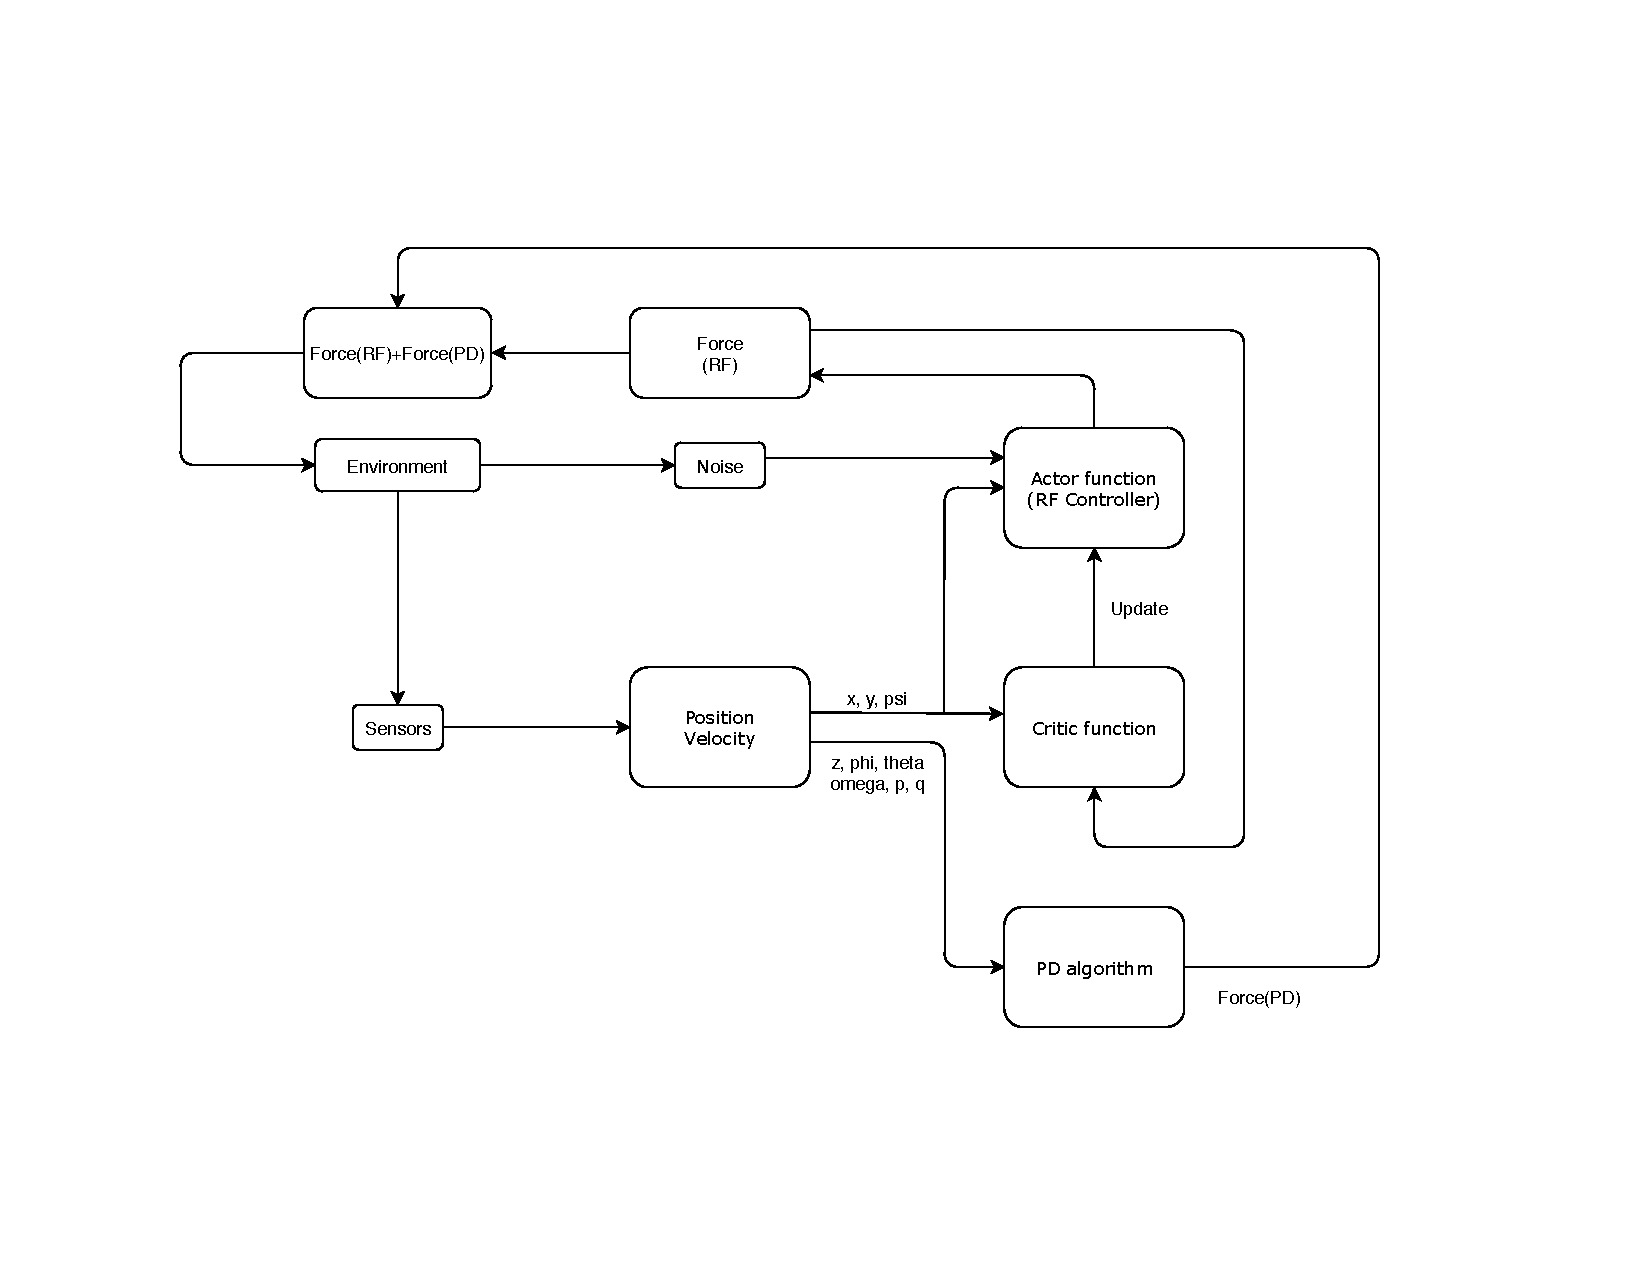
\includegraphics[width=\textwidth, trim={1cm 4cm 1cm 3cm},clip]{images/chap4/architecture.pdf}
    \caption{Controller Architecture for the BlueROV2}
    \label{fig:architecture}
\end{figure}
From the BlueRov2s' sensors the controller receives the positions and velocities in the given states. The PD algorithm will then receive the position states $z, \phi, \theta$ and the velocity states $\omega, p, q$ to calculate the needed force input in $z, \phi$ and $\theta$. At the same time-step the Reinforced Learning algorithm will receive the position states $x, y, \psi$ to calculate the needed force input in these states. This results in the force input matrix in the given state, $s_{t}$, being equal to
\begin{equation}
    \tau = \begin{bmatrix}
    \tau_{x} \\ \tau_{y} \\ \tau_{z} \\ \tau_{\phi} \\ \tau_{\theta} \\ \tau_{\psi}
    \end{bmatrix}
\end{equation}
The Reinforced Learning algorithm is displayed in Algorithm \ref{alg:RF}. As shown in the algorithm it clips the action, $a_{t}$, based on $a_{t} \in [-1 , 1]$ and a factor $\epsilon$. $\epsilon$ is here the exploitation versus exploration factor, discussed in chapter \ref{chap:station-keeping}. Both networks also need to be discounted by a \textit{learning rate} $\alpha$, which says something about how much the algorithm values new information in a given state versus the learned optimal actions in that state. The learning rate should also be decreased over the number of iterations, since the algorithm gains larger and lager knowledge about the environment.\\
\begin{algorithm}[H]
\SetAlgoLined
    Initialise the network classes $Q(s_{t},a_{t}|\omega)$ and $\mu(s_{t}|\omega)$ with weights $\omega$ and $\theta$.\\
    Initialise the replay buffer R as a memory class, M, to hold $s_{t}, a_{t}, r_{t}$ and $s_{t+1}$.\\
    \For{ep \textbf{in} MAX\_EPISODES}{
    Initialise episode reward to zero\\
    Initialise episode step, $t$, to zero\\
    \While{t $<$ MAX\_EP\_STEPS}{
    Initialise desired state, $s_{d}$\\
    Initialise desired state PID, $s_{d,PD}$\\
    get position states, $x, y, z$, and orientation states, $\epsilon_{1}, \epsilon_{2}, \epsilon_{3}, \eta$\\
    get the Euler angles $\phi, \theta, \psi$ from the orientation states\\
    compute $s_{t}=(x, y, \psi)$\\
    Choose action $a_{t}=\mu(s_{t}|\theta)$\\
    clip action based on $a_{max}, a_{min}$ and $\epsilon$\\
    compute the error state, $s_{e}$\\
    compute the error state PID, $s_{e, PID}$\\
    compute $r(s_{t},a_{t})$\\
    episode reward += $r(s_{t},a_{t})$\\
    store in transition $R(s_{t},a_{t},r_{t},s_{t+1})$\\
    Randomly select N arrays from R\\
    compute $y_{i}=r_{i}+\gamma Q(s_{i},a_{i}|\omega)$\\
    compute $Loss=\frac{1}{N}\sum_{i=1}^{N}(y_{i}-Q(s_{i},a_{i}|\omega))^{2}$\\
    compute $\nabla_{\omega}Loss=\frac{1}{N}\sum_{i=1}^{N}(y_{i}-Q(s_{i},a_{i}|\omega))\frac{\partial Q(s_{i},a_{i}|\omega)}{\partial \omega}$\\
    update weight $\omega_{t+1}=\omega_{t}+\alpha\nabla_{\omega}Loss$\\
    compute $\nabla_{\theta}J=\frac{1}{N}\sum_{i=1}^{N}\frac{\partial Q(s_{i},a_{i}|\mu(s_{i}|\theta))}{\partial a_{i}}\frac{\partial \mu(s_{i}|\theta)}{\partial\theta}$\\
    compute $m_{t}=\wp\times m_{t-1}+(1-\wp)\nabla_{\theta}\mu$\\
    compute $\Im_{t} & = \beta\times\Im_{t-1}+(1-\beta)\nabla_{\theta}\mu$\\
    compute $\Hat{m}_{t} & = \frac{m_{t}}{1-\wp^{t}}$\\
    compute $\Hat{\Im}_{t} & = \frac{\Im_{t}}{1-\beta^{t}}$\\
    update weight $\theta_{t+1} & = \theta_{t} - \eta\frac{1}{\sqrt{\Hat{\Im}_{t}}}\Hat{m}_{t}$\\
    update weight $\omega^{'}=\rho\omega+(1-\rho)\omega^{'}$ ($\rho$ is learning rate)\\
    update weight $\theta^{'}=\rho\theta+(1-\rho)\theta^{'}$\\
    Get velocity states $[\omega_{t}, p_{t}, q_{t}$]\\
    Get $\tau_{PID}$ from velocity states and $s_{t,PD} = [z, \phi, \theta]$\\
    Set the output thrust equal to: $\tau[0,1,5]=a_{t}$ and $\tau[2,3,4]=\tau_{PD}$\\
    }
    }
\caption{DDPG algorithm}
\label{alg:RF}
\end{algorithm}

\subsection{Reward function}
Optimal design of the reward function, $r(s_{t},a_{t})$, is essential for the behaviour of the algorithm. As mentioned throughout this paper, the reward is a feedback from the environment based on how good it was to take a particular action in a given state. The agent is continuously looking for the highest total cumulative reward, in order to determine the optimal policy starting in any state. Because of this, different reward function designs have been tested, more about this in the next chapter. 
\section{Software}
In order to evaluate the controller design the simulators \textbf{Gazebo} and \textbf{Robotic Operating System} (ROS) were used. Gazebo, which offers the ability to accurately and efficiently simulate a robotic system in complex environments, was used to simulate the \textit{MC Lab} at \textit{Marin Teknisk Senter} in Trondheim, Norway. ROS was used to simulate the dynamics of the \textbf{BlueROV2}, and combining these two resulted in the simulator in figure \ref{fig:ros}. 
\begin{figure}[H]
    \centering
    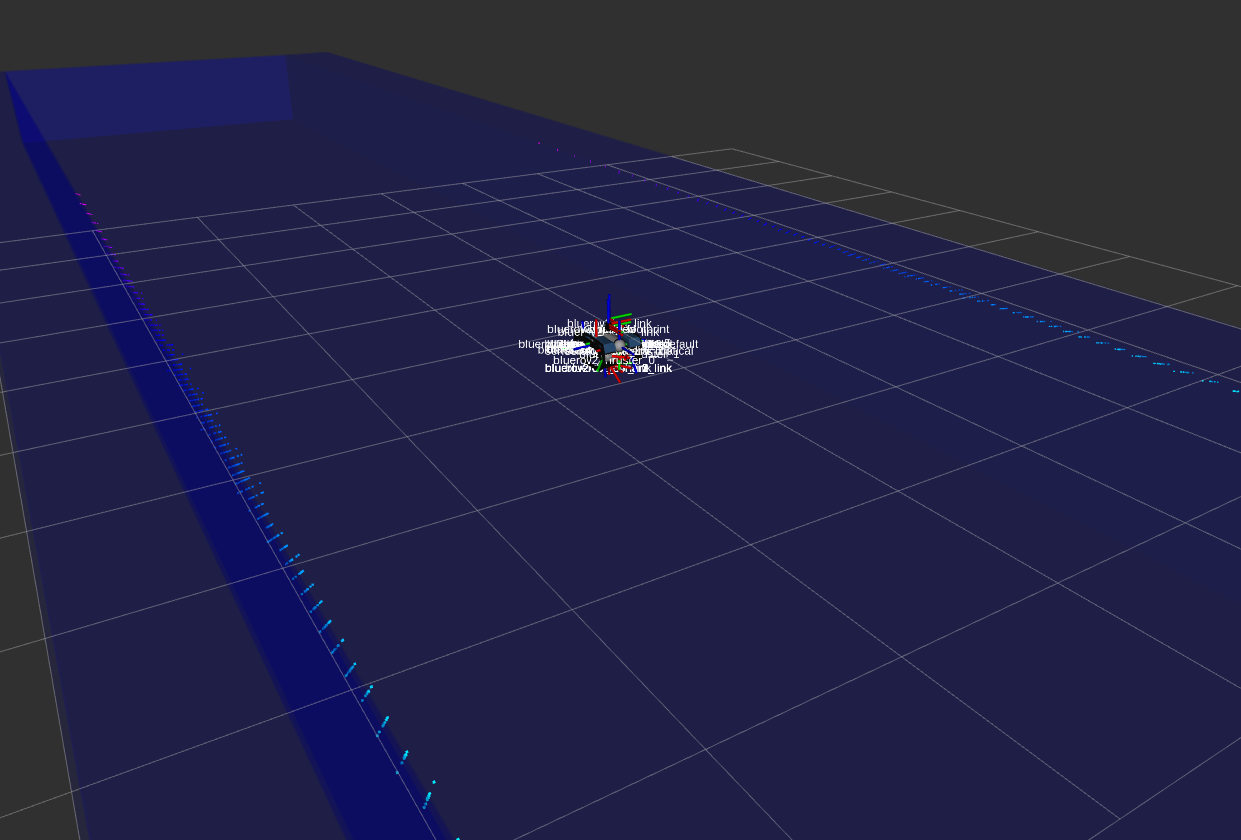
\includegraphics[width=0.7\textwidth]{images/chap4/ROS.png}
    \caption{Gazebo and Robotic Operating System (ROS) with the BlueROV2 AUV}
    \label{fig:ros}
\end{figure}
For the implementation of the controller design, both the DP algorithm and the DDPG algorithm, the programming framework \textbf{TensorFlow} was chosen. TensorFlow is an open-source machine learning framework, which works well in combination with the \textbf{Python} programming language. 

\chapter{Simulation results}
As discussed in chapter \ref{chap:method} the PD algorithm was initially tuned to make sure that the states ($\phi, \theta, z$) were stable on their own. This was done by giving the vehicle a fixed thrust in the $x$ direction, which resulted in the following proportional and derivative gains
\begin{align}
    K_{p} & = 1 \\
    K_{d} & = 0.1
\end{align}
In order to sufficiently train the DDPG algorithm the simulation was executed over $N = 400$ episodes, where each episode consisted of $t = [1, T=1000]$ steps. For each episode the algorithm will therefore be executed until T = 1000 \textbf{or} the BlueROV2 reaches the terminal state, indicating the it has reached the desired pose. The reward discount factor ($\gamma$), learning rate for the actor network ($\alpha_{a}$), learning rate for the critic network ($\alpha_{q}$) and the exploitation/exploration factor ($\epsilon$) were initially defined as
\begin{align}
    \gamma & = 0.9 \\
    \alha_{a} & = 1e-4 \\
    \alpha_{q} & = 1e-4 \\
    \epsilon & = 1
\end{align}
Recall $\alpha_{a}, \alpha_{q}$ and $\epsilon$ should all decrease over the number of iteration, since the algorithm gains larger and larger knowledge about the environment. This was by discounting the parameters at each episode, $N_{i}$ $(i = 1,...,400)$.\\\\
To accomplish Station Keeping the desired pose were defined as
\begin{align}
    s_{d} & = [x_{d}, y_{d}, \psi_{d}] = [1, 1, 0] \\
    s_{d,PD} & = [z_{d}, \phi_{d}, \theta_{d}] = [0, 0, 0]
\end{align}
Meaning that the BlueROV2 should stabilise at [$x = 1, y = 1$] in (NED).  
\section{Simulation 1}
As mentioned in chapter \ref{chap:method}, the reward function design is critical for the performance of the algorithm. Initially the reward function was defined with respect to the BlueROV2s' distance to the desired state, meaning that a larger distance should give a lower reward. The reward function, $r(s_{t}, a_{t})$, was therefore defined as
\begin{align}
    r(s_{t}, a_{t}) & = \frac{1}{\norm{s_{e}}} \\
    s_{e} & = s_{d} - s_{t} \\
    R_{N_{i}} & += r(s_{t}, a_{t})
\end{align}
where $R_{N_{i}}$ is the total reward over episode $N_{i}$, where $i=1,..,N$. Because of uncertainty in the measurements a vector consisting of the mean value over the 100 latest total rewards, $[R_{N_{i-100}},...,R_{N_{i}}]$, was defined. By plotting this vector over $N$ episodes the following result was obtained
\begin{figure}[H]
    \centering
    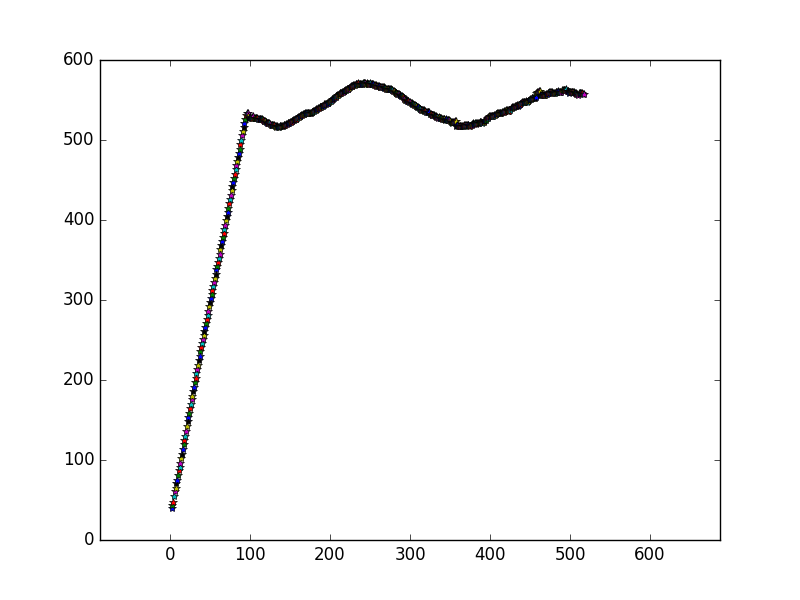
\includegraphics[width=0.7\textwidth]{images/chap5/figure_1.png}
    \caption{Simulation 1}
    \label{fig:sim1}
\end{figure}
In figure \ref{fig:sim1} the $y-axis$ specifies the total reward, and the $x-axis$ specifies number of episode. From the figure we see that the total reward converges to an oscillating value. Since the figure displays the mean value over the 100 latest episodes it is expected that the graph converges to a constant value, because the algorithm should learn the optimal action to take in every state, which results in the total reward being constant in each episode after it has learned the optimal behaviour. However, as previously stated the episodes is defined in such a way that the algorithm will be executed until T = 1000, or the BlueROV2 reaches the terminal state. This means that although it receives the highest reward at the desired position the episode will also terminate at this position, meaning that it will receive a larger total reward, $R_{N}$, by circulating the desired pose for $t=[1,T]$. This shows the importance of the reward function design, since the algorithm is able to find the optimal policy in each state, but the framework defined by the reward function is not optimal. 
\section{Simulation 2}
From the knowledge gained in simulation 1 it was clear that the reward function needed to be redesigned, in order to compensate for the fact that the algorithm received larger rewards for circulating the desired pose compared to reaching the terminal state. The new reward function was therefore defined as

\begin{algorithm}[H]
\SetAlgoLined
\begin{align}
    r(s_{t}, a_{t}) & = \frac{1}{\norm{s_{e}}} \\
    r(s_{t}, a_{t}) & += -0.05*t
\end{align}
    \If{abs($s_{e}$[0]) $<$ 0.1 \textbf{and} abs($s_{e}$[1]) $<$ 0.1}{
    r += 20 \\
    done = \textbf{True}
    }
    \If{$s_{e, diff}$[0] $<$ 0 \textbf{and} abs($s_{e, diff}$[1]) $<$ 0}{
    r += -5
    }
\caption{Reward function}
\label{alg:reward_func}
\end{algorithm}
The algorithm now receives a negative reward, or a penalty, at each step $t$, meaning that it accomplishes the greatest total reward when reaching the desired pose using minimum steps. This will therefore prevent circulating the desired pose being the optimal behaviour. In algorithm \ref{alg:reward_func} I have included two if-sentences, where the first one checks the absolute error in the $x-$ and $y$ position. The reason for neglecting the error in $\psi$ here is that this state is valued less than the other two states. For Station Keeping the $x-$ and $y$ positions are more "\textit{relevant}". The second if-sentence evaluates $s_{e,diff}$, which is defined as the difference between the current error values and the error values in the previous step, $t-1$. If this difference is negative it means that the AUV moves away from the desired pose, which results in an additional penalty. 
\begin{figure}[H]
    \centering
    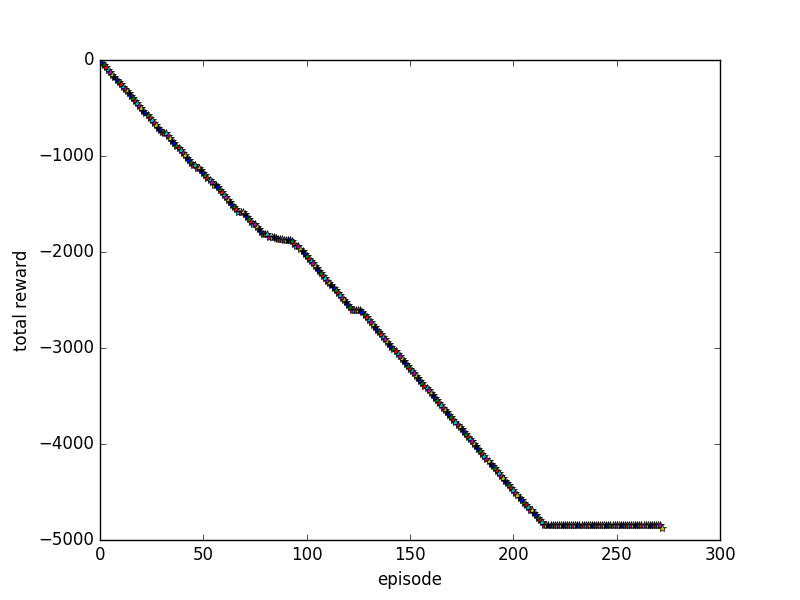
\includegraphics[width=0.7\textwidth]{images/chap5/figure_1-1.png}
    \caption{Simulation 2}
    \label{fig:sim2}
\end{figure}
The result from simulation 2 is illustrated in figure \ref{fig:sim2}. Here we see that the algorithm converges to a constant total reward of $\approx$ -4800 after $\approx$ 215 episodes. Compared to simulation 1 the oscillating behaviour is removed, and the algorithm has successfully learned the optimal behaviour for Station Keeping at the desired pose. 
\chapter{Conclusion}
This report has investigated the use of \textit{Deep Learning} techniques in \textit{Station Keeping} of underwater vehicles. Traditional methods of Station Keeping have been presented, and it was discussed how Deep Learning techniques could solve the problems related to pose estimation and underwater control. A literature review was conducted on the topics of \textit{machine learning} and \textit{visual servoing}. This revealed that the underwater environment can be defined as a \textit{Markov Decision Process}, which showed that underwater control problems is \textit{solvable} through the use of \textit{Reinforcement Learning}. Investigating the research done on the topic of visual servoing it was revealed that \textit{Convolutional Neural Networks} have showed the most promising results for implementation of visual servoing in underwater robotics.\\\\
In the second part of the report a development of a state-of-the-art \textit{Deep Deterministic Policy Gradient} controller for underwater control was conducted. By investigating the dynamics, kinematics and hydrodynamics of the BlueROV2 it was revealed that a combination of a \textit{PD} controller with the \textit{DDPG} controller could be a possible solution to achieve Station Keeping in \textit{all} 6 DOFs for the vehicle.\\\\
By using the \textit{Gazebo} and \textit{ROS} simulation environments, the results showed that the DDPG algorithm was successful in finding the optimal policy to reach the desired pose in all 6 DOFs. The simulations also revealed the importance of optimal design of the \textit{reward function}, which in all simplicity sets the operation framework for the vehicle. As stated throughout this study, the DDPG algorithm is always looking for the policy that results in the highest total cumulative reward. This means that the algorithm will always discover possible "flaws" in the framework definitions, that the human eye might not see. From the simulation results this was revealed when evaluating the performance of algorithm \ref{alg:reward_func_2}. The algorithm was successfully in reaching the desired pose, but had no stored policy for which actions to execute after reaching this state. This was due to the definition of the \textit{terminal state}, and a possible action to resolve the problem was to include \textit{time} constraints in the reward function. 

\chapter{Conclusion}
\section{Further Work}

\printglossary[type=\acronymtype,title=Acronyms]

\newpage
\bibliographystyle{plain}
\bibliography{biblist}
\newpage
\appendix
\chapter{BlueROV2 Parameters}
The following matrices are extracted from \textit{BlueRobotics} \cite{blue}.
\section{Rigid Body Mass Matrix}
\begin{equation}
    \mathbf{M}_{RB} = - \begin{bmatrix}
    10.5 & 0 & 0 & 0 & 0 & 0 \\
    0 & 10.5 & 0 & 0 & 0 & 0 \\
    0 & 0 & 10.5 & 0 & 0 & 0 \\
    0 & 0 & 0 & 0.156 & 0.003 & -0.006 \\
    0 & 0 & 0 & 0.003 & 0.214 & 0.004 \\
    0 & 0 & 0 & -0.006 & 0.004 & 0.127 \\
    \end{bmatrix}
\end{equation}
\section{Added Mass Matrix}
\begin{equation}
    \mathbf{M}_{A} = - \begin{bmatrix}
    7.0377 & -1.2910 & -1.6817 & 0.0954 & 0.2690 & -0.0563 \\
    0.5638 & 18.5399 & 0.9321 & 0.193 & -0.1080 & -0.1984 \\
    2.6036 & 8.6394 & 13.2816 & -0.5730 & -1.7952 & 0.2603 \\
    0.0587 & 0.2892 & 0.0834 & 0.0546 & -0.0087 & -0.0284 \\
    0.1266 & 0.1660 & 0.1468 & -0.0124 & 0.0173 & 0.0044 \\
    -0.0621 & -0.2041 & -0.0711 & -0.0168 & 0.0061 & 0.2795 
    \end{bmatrix}
\end{equation}
\section{Damping Matrices}
\begin{align}
    \mathbf{D}_{L} & = -diag\{0, 0.26, 0.19, 0.895, 0.287, 4.64\} \\
    \mathbf{D}_{Q} & = -diag\{3.96|u|, 103.25|v|, 74.23|\omega|, 0.084|p|, 0.028|q|, 0.43|r|\}
\end{align}

\end{document}